\chapter{Input variables to the neural network in the \ttH\ analysis}
\label{app:separation}

Figures~\ref{fig:sepinput_lj_0}--\ref{fig:sepinput_lj_3}
show the discrimination between 
signal and background for the top four input variables in each region 
where NN is used.
In the \fivethree\ region, the NN is designed to separate $t\bar{t}$+HF from $t\bar{t}$+light.
Comparisons between data and post-fit predictions for the most discriminating variables can be found in figures~\ref{fig:postinput_lj_0} --\ref{fig:postinput_lj_3}.

\begin{figure}[tp]
\begin{center}
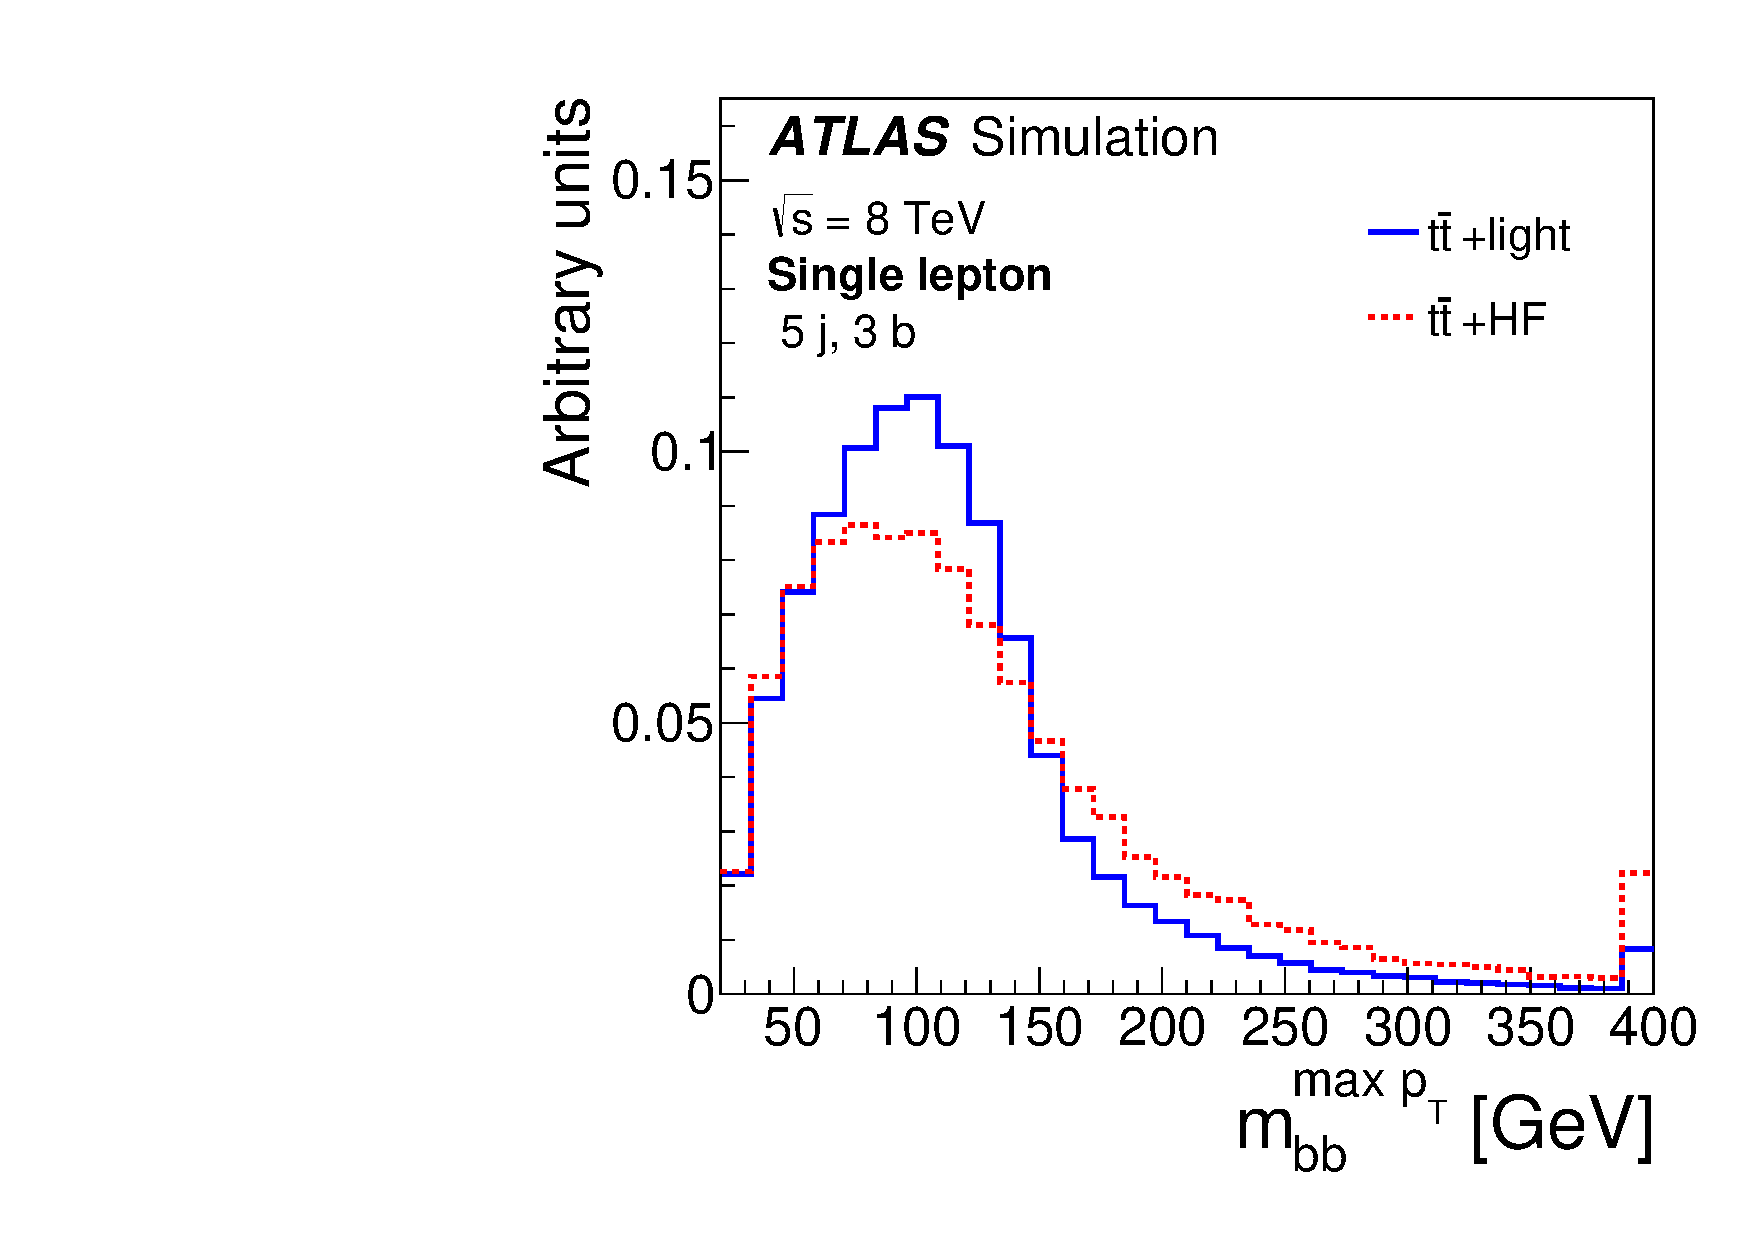
\includegraphics[width=0.49\textwidth]{Appendices/Figures_separation/mbb_maxPt_5_flav.pdf}
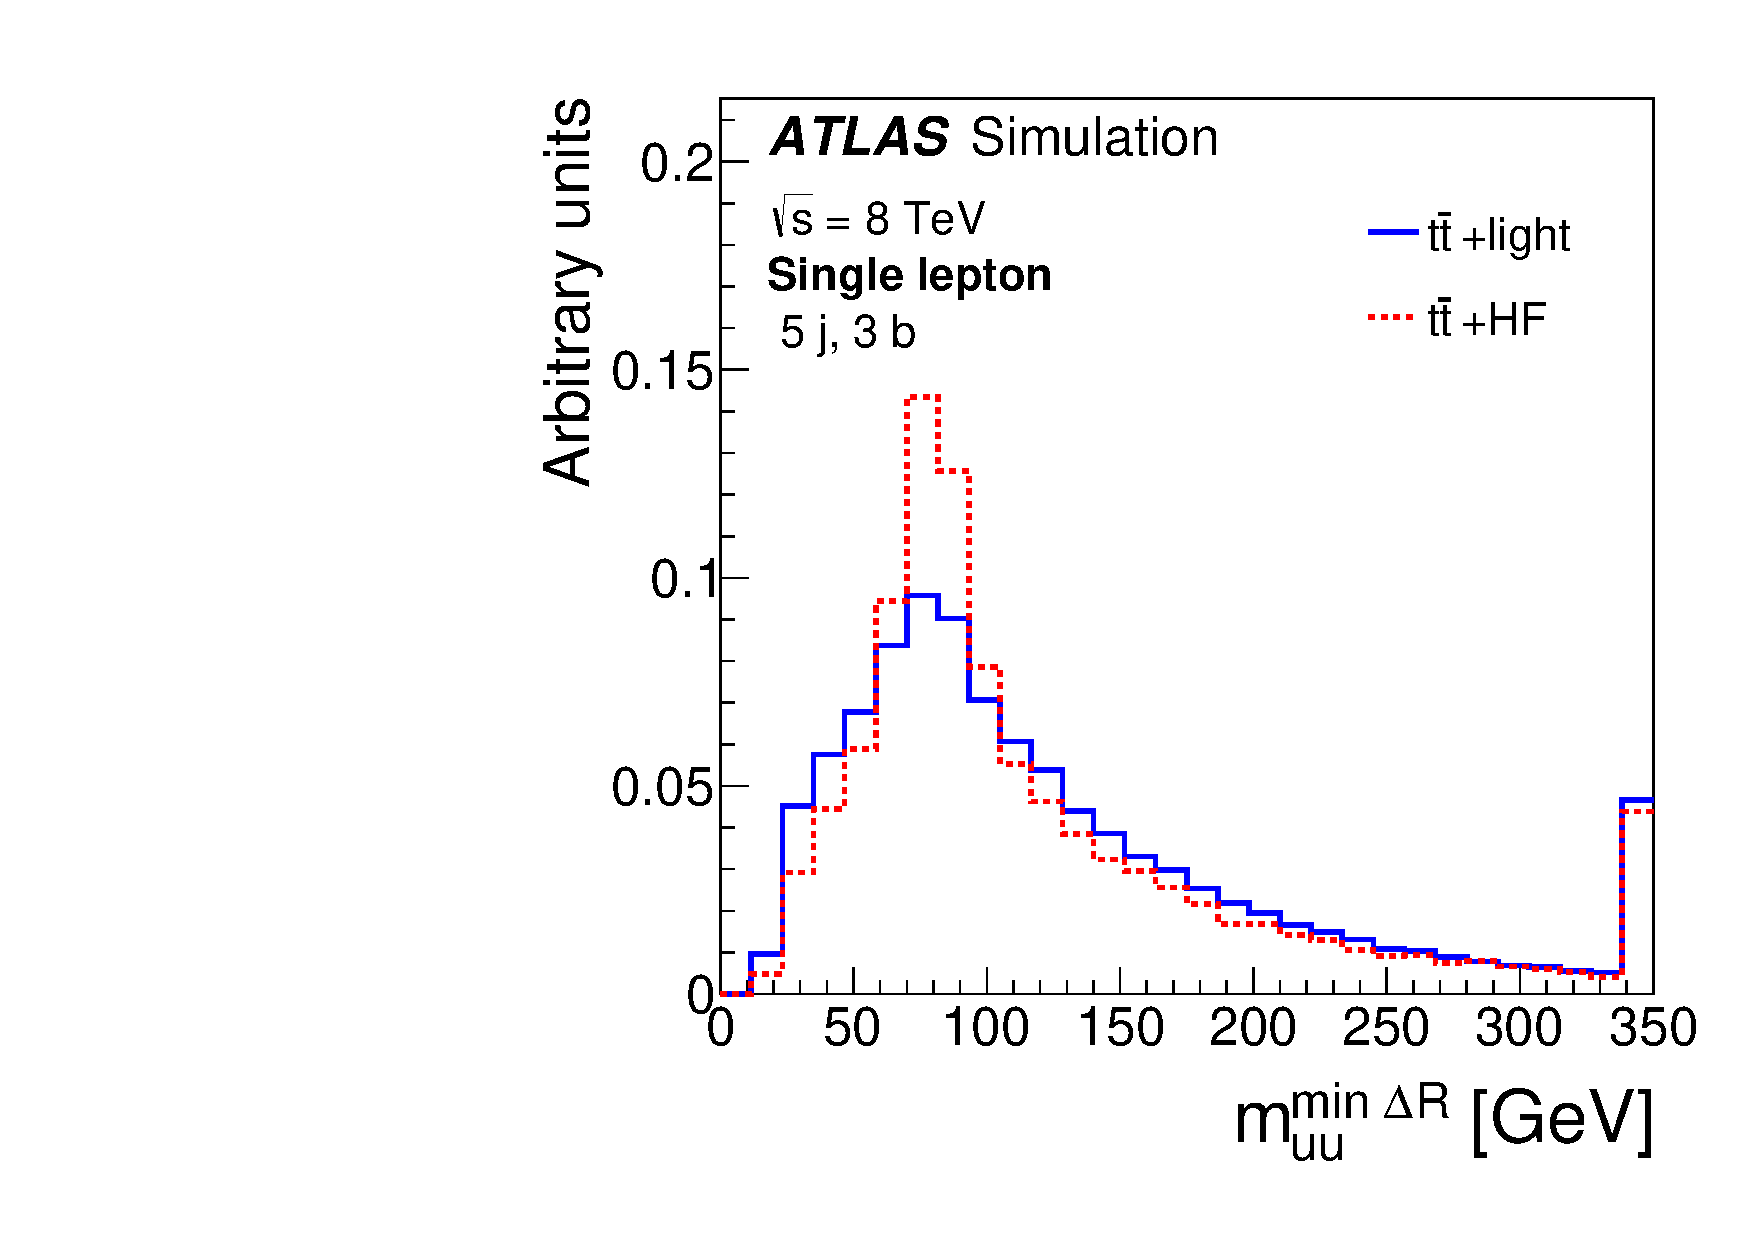
\includegraphics[width=0.49\textwidth]{Appendices/Figures_separation/WhadM_5_flav.pdf} \\
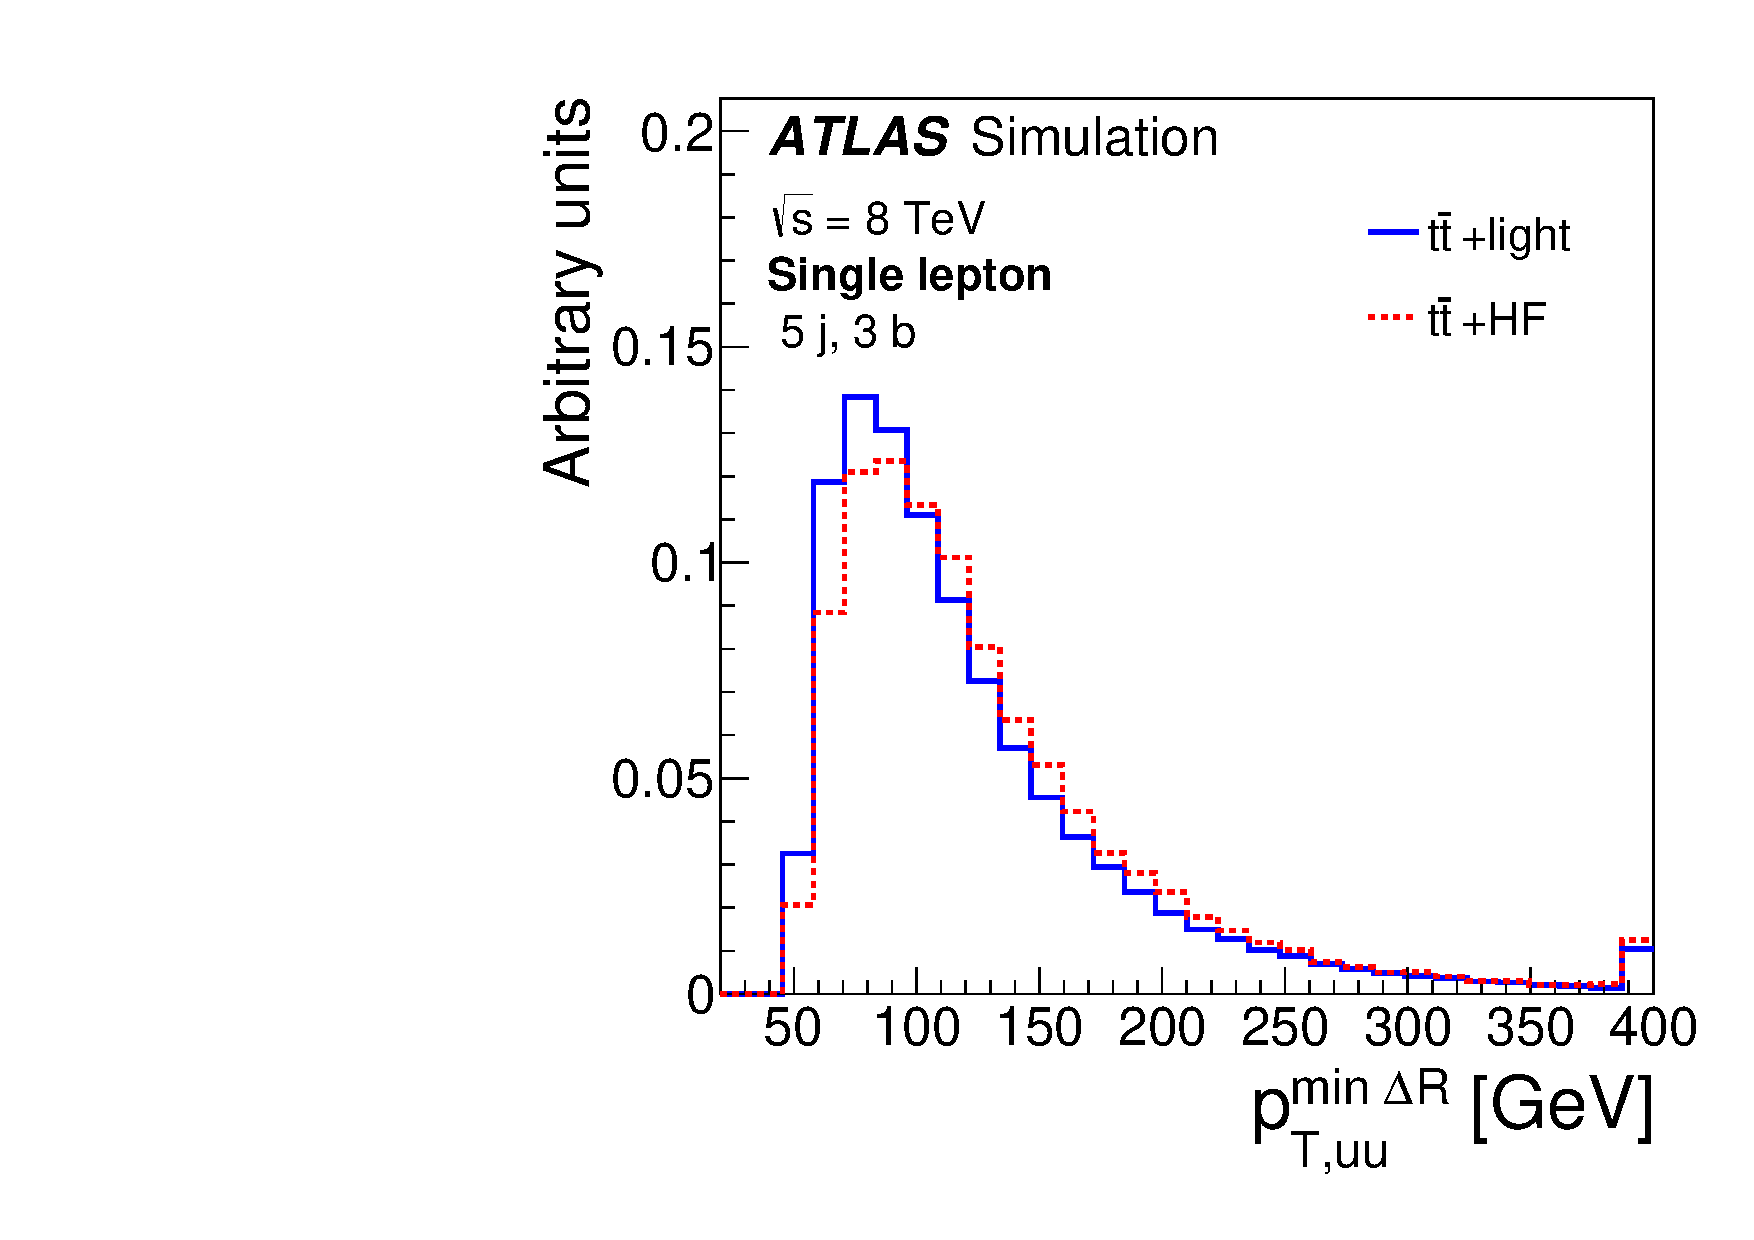
\includegraphics[width=0.49\textwidth]{Appendices/Figures_separation/WhadSpt_5_flav.pdf}
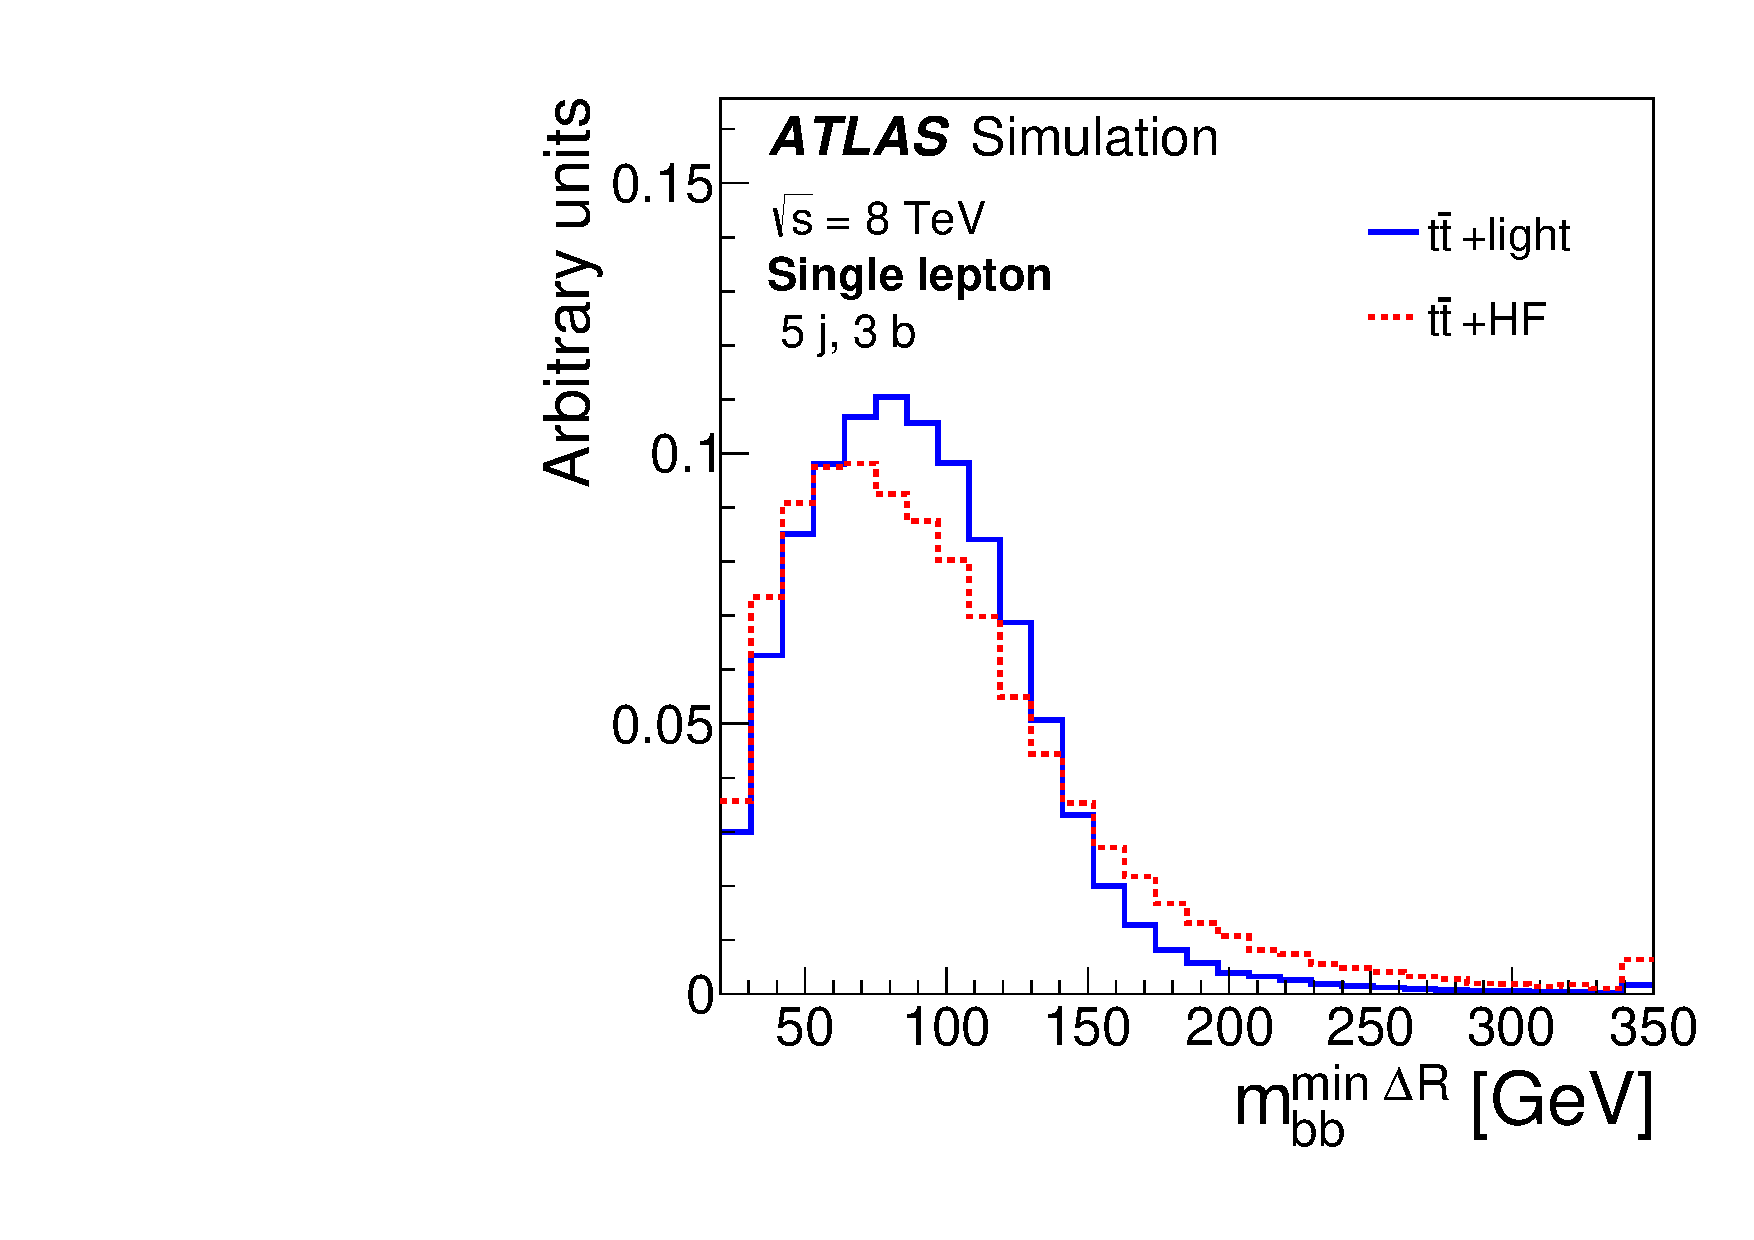
\includegraphics[width=0.49\textwidth]{Appendices/Figures_separation/mbb_mindR_5_flav.pdf}
\caption{Comparison of $t\bar{t}$+HF (dashed) and $t\bar{t}$+light (solid) background for the four top-ranked 
input variables in the \fivethree\ region where the NN is designed to separate these two backgrounds. 
The distributions shown are (a) \mbbmaxpt, (b) \whadmass, (c)  \whadpt and (d) \mbbmindr.
}
\label{fig:sepinput_lj_0} 
\end{center}
\end{figure}

\begin{figure}[tp]
\begin{center}
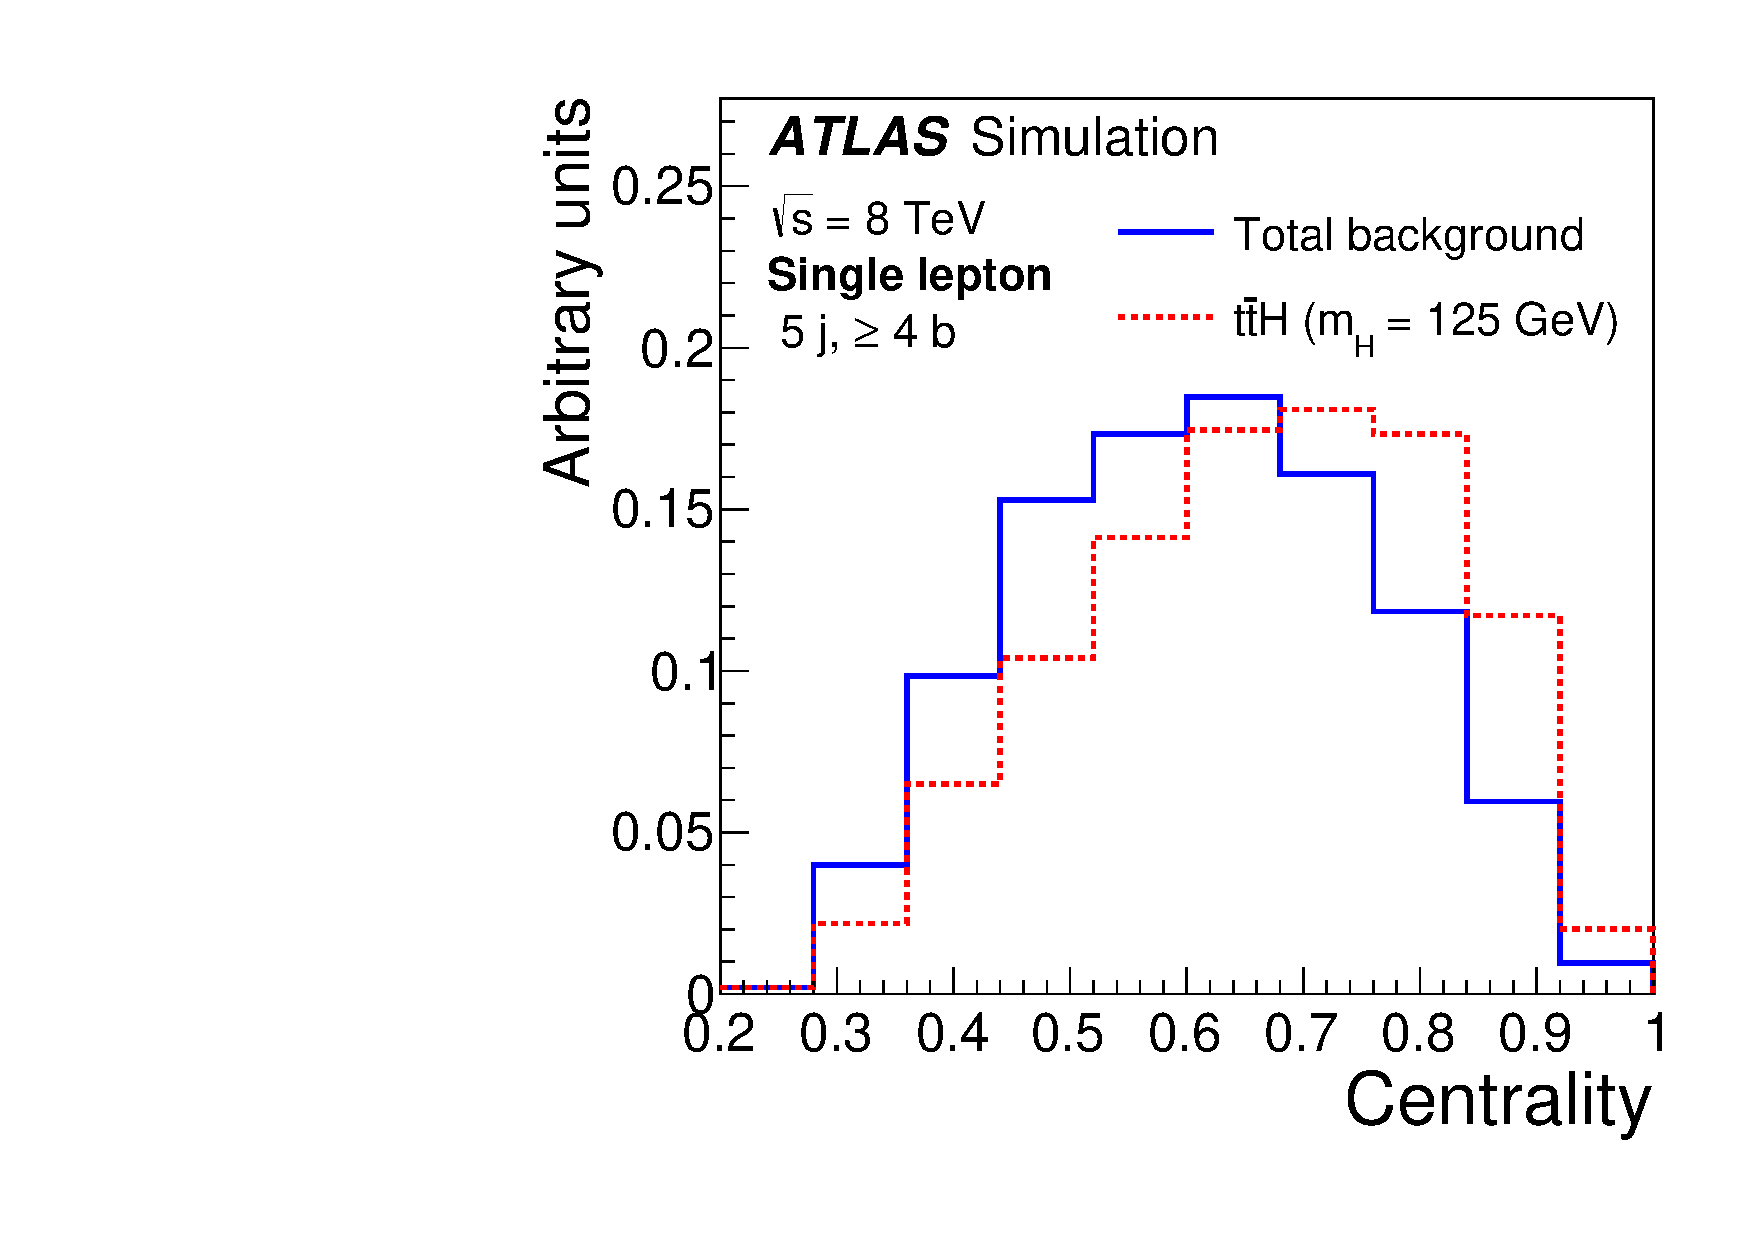
\includegraphics[width=0.49\textwidth]{Appendices/Figures_separation/cent_5_sep.pdf}
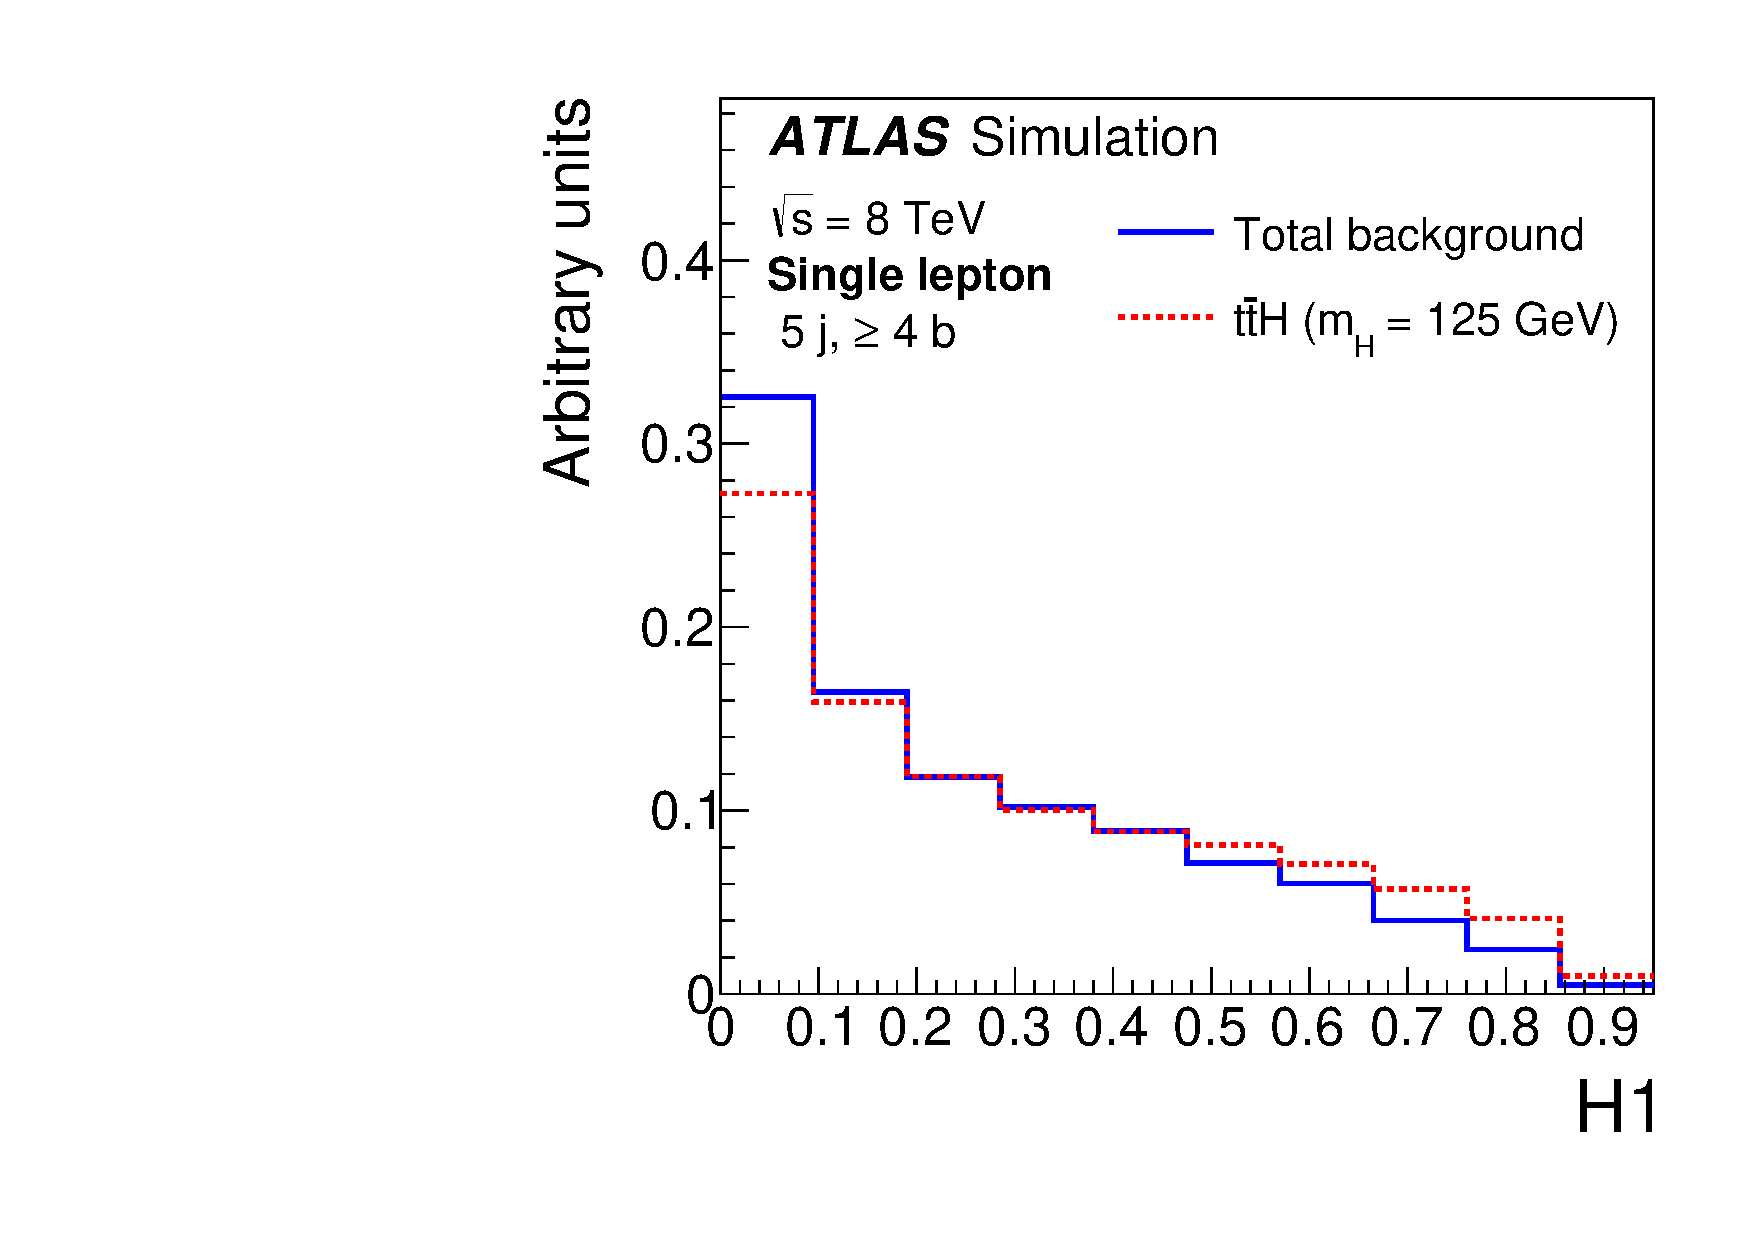
\includegraphics[width=0.49\textwidth]{Appendices/Figures_separation/H1_5_sep.pdf}\\
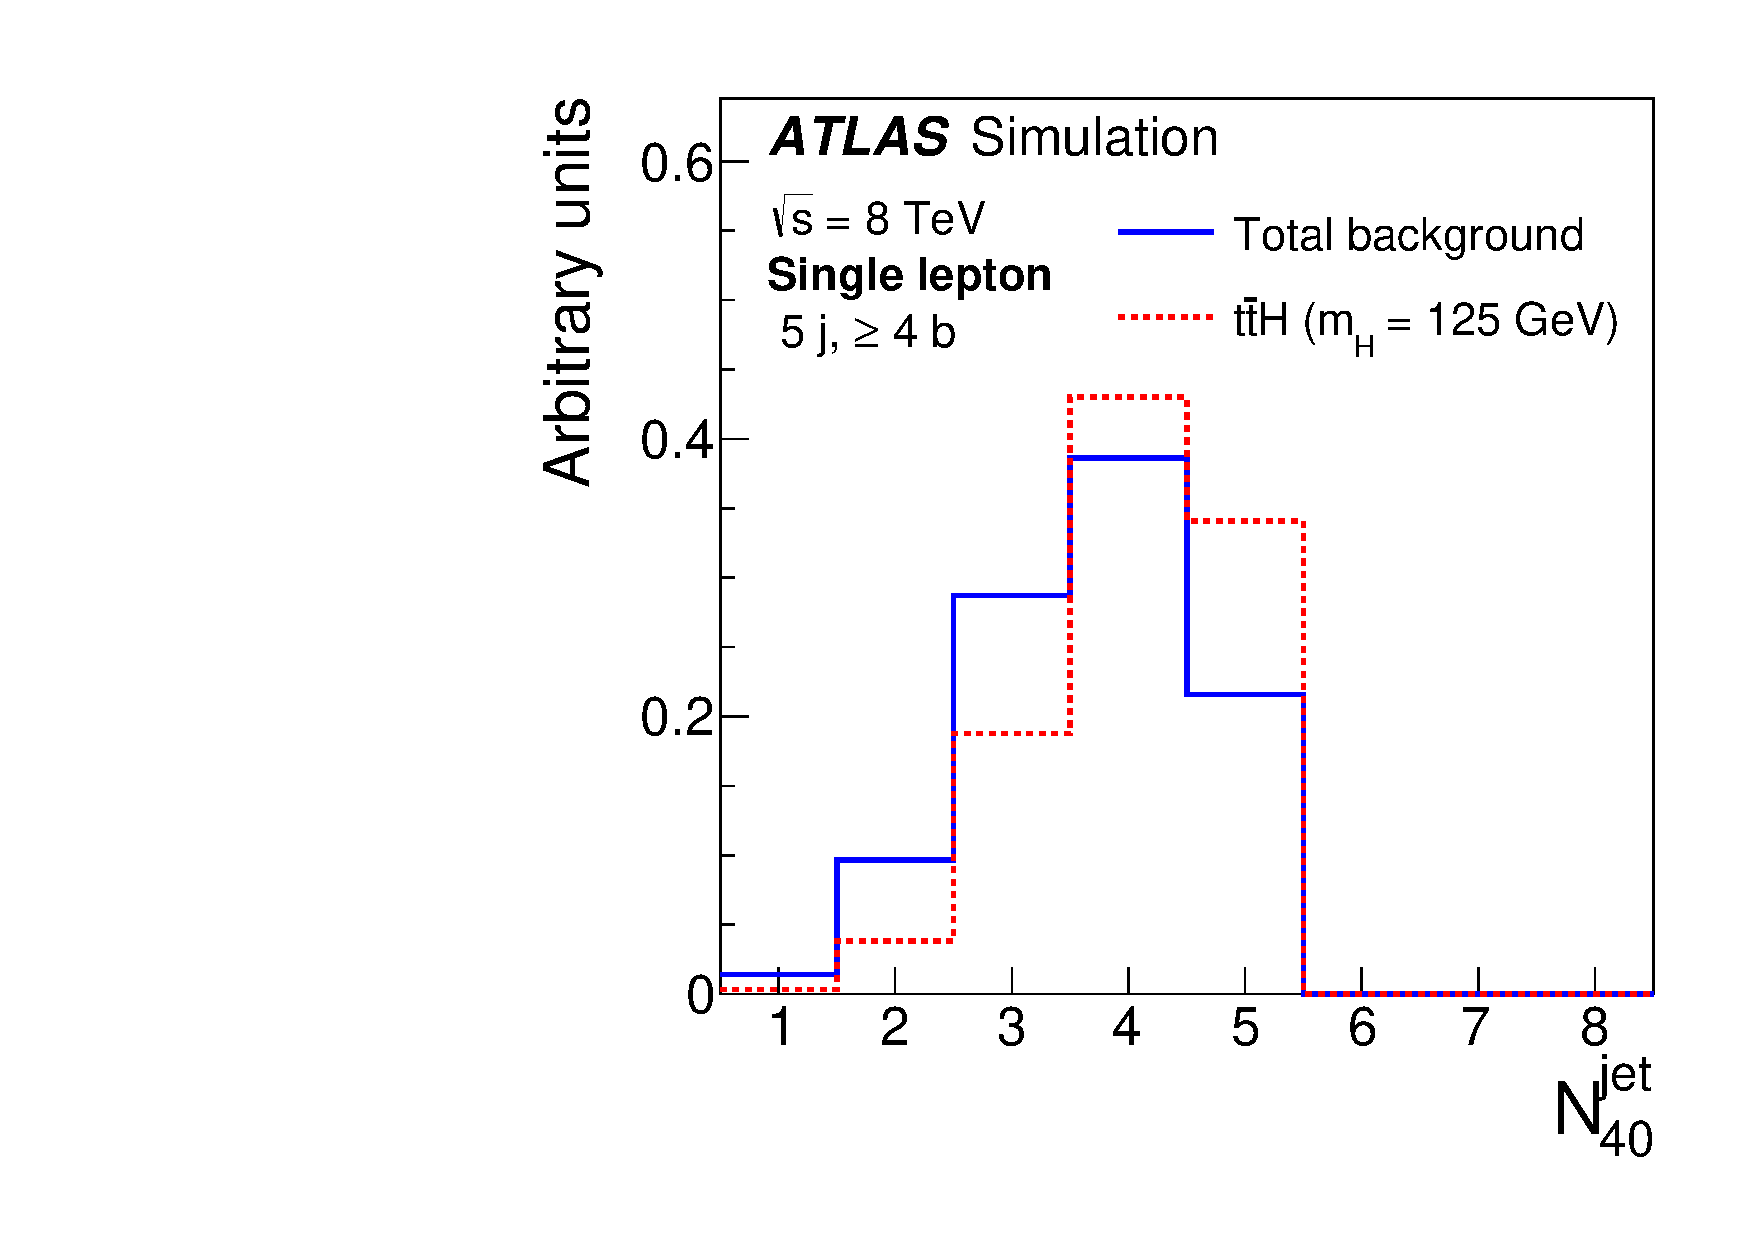
\includegraphics[width=0.49\textwidth]{Appendices/Figures_separation/num_jet_40_5_sep.pdf}
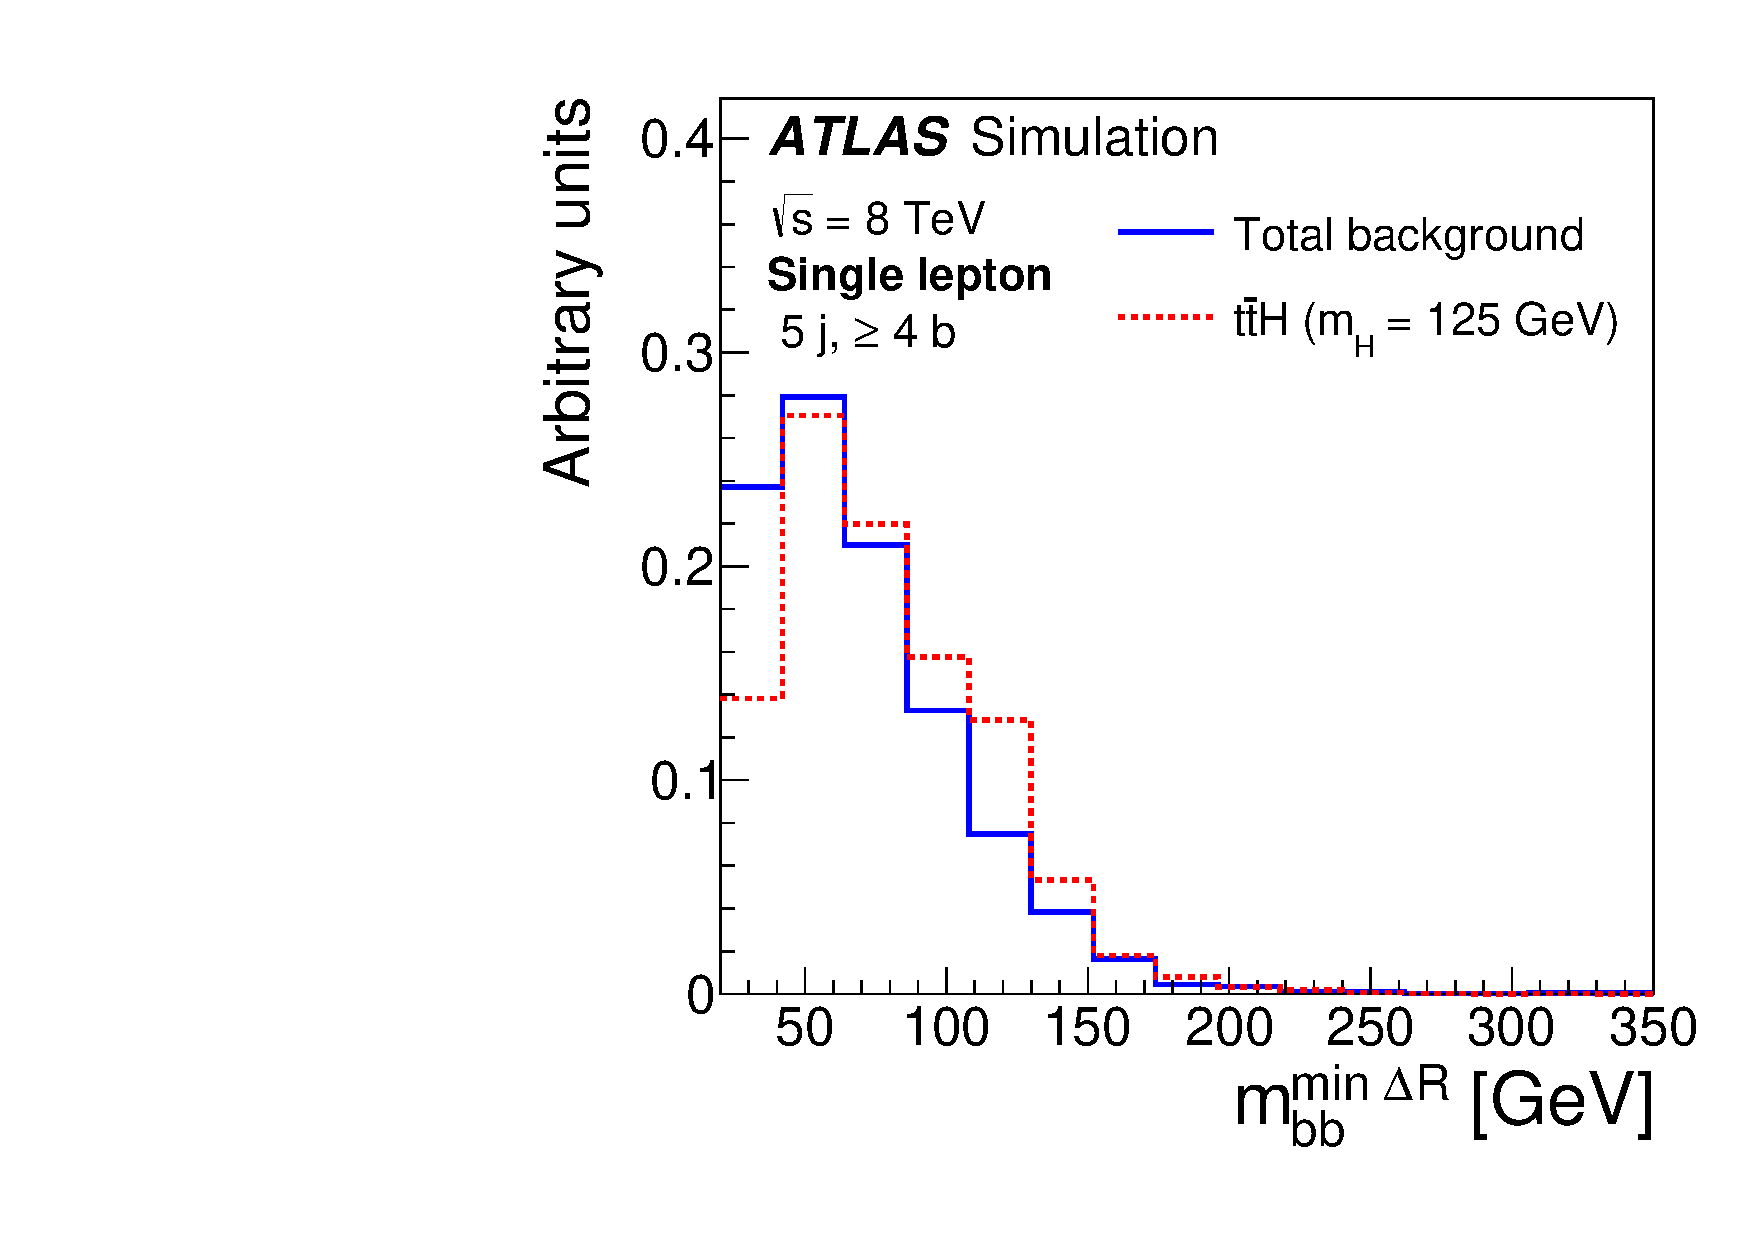
\includegraphics[width=0.49\textwidth]{Appendices/Figures_separation/mbb_mindR_5_sep.pdf}
\caption{Comparison of \tth\ signal (dashed) and background (solid) for the four top-ranked input variables in the 
\fivefour\ region.  The distributions shown are (a) \cent, (b) $H1$, (c)  \numjetforty and (d) \mbbmindr.
}
\label{fig:sepinput_lj_1} 
\end{center}
\end{figure}

\begin{figure}[tp]
\begin{center}
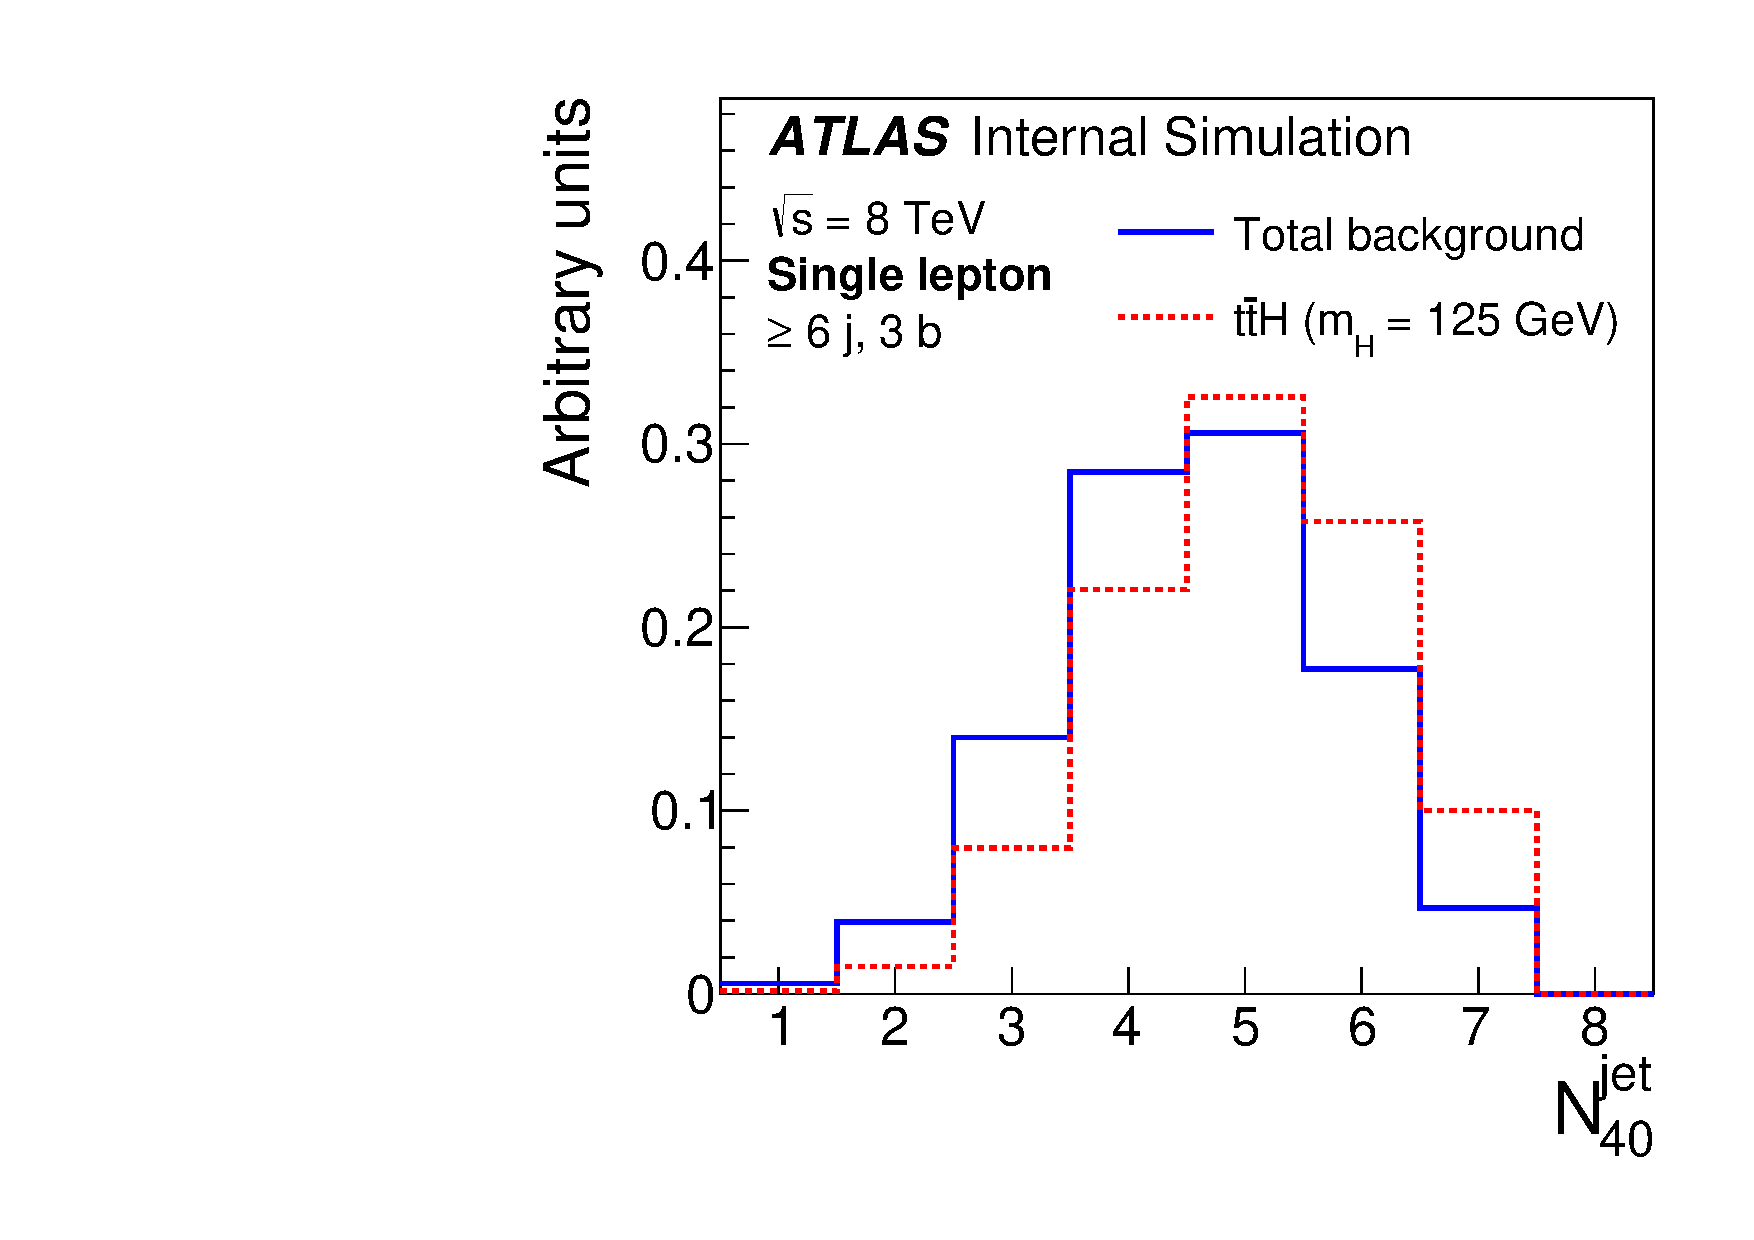
\includegraphics[width=0.49\textwidth]{Appendices/Figures_separation/num_jet_40_6jincl_sep5.pdf}
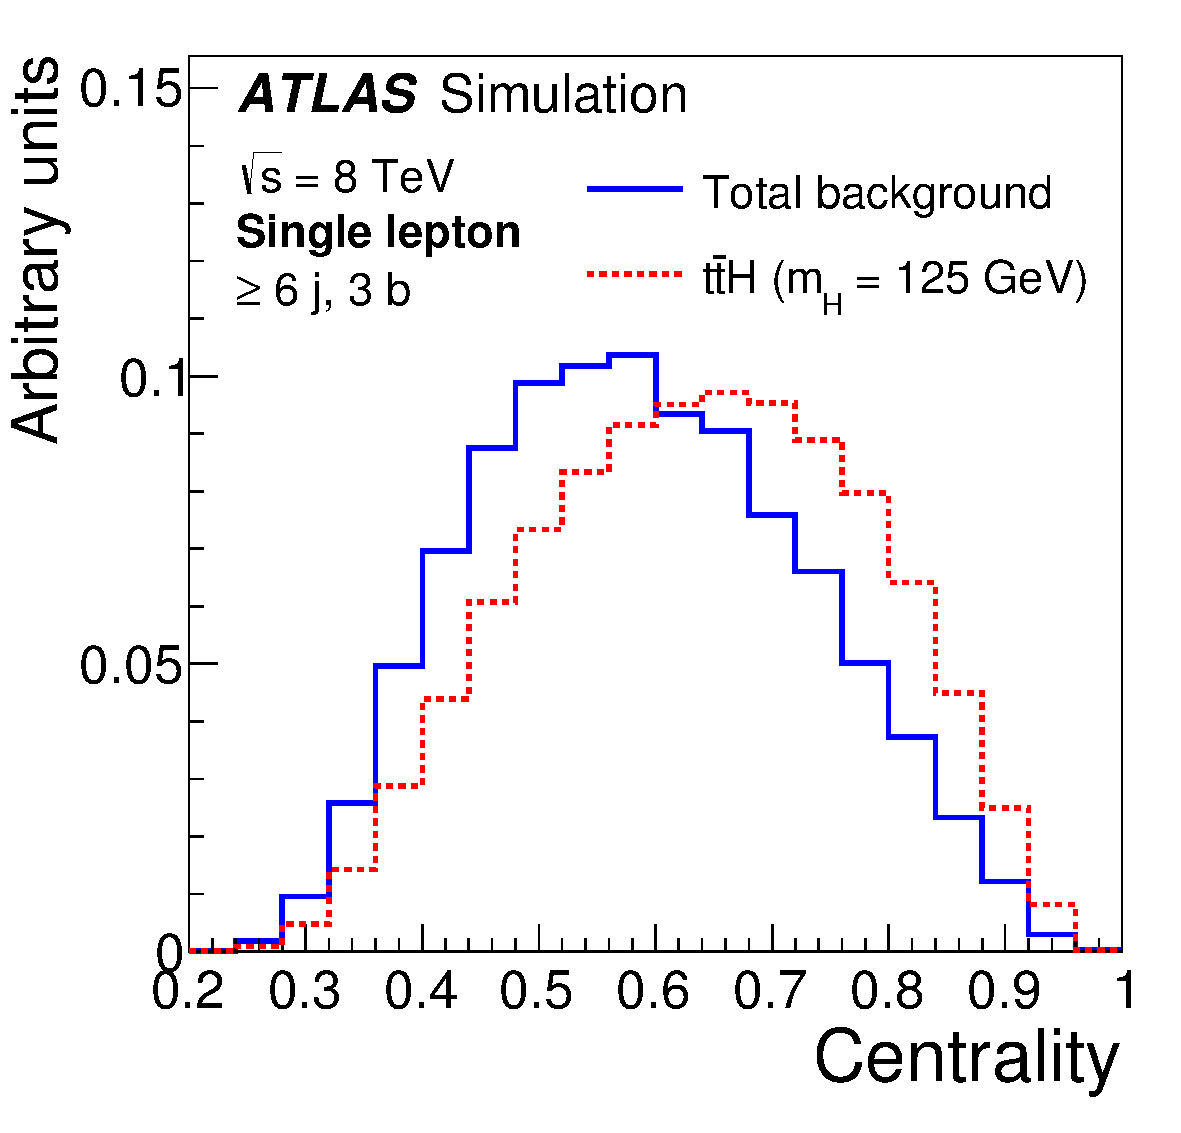
\includegraphics[width=0.49\textwidth]{Appendices/Figures_separation/cent_6jincl_sep5.pdf}\\
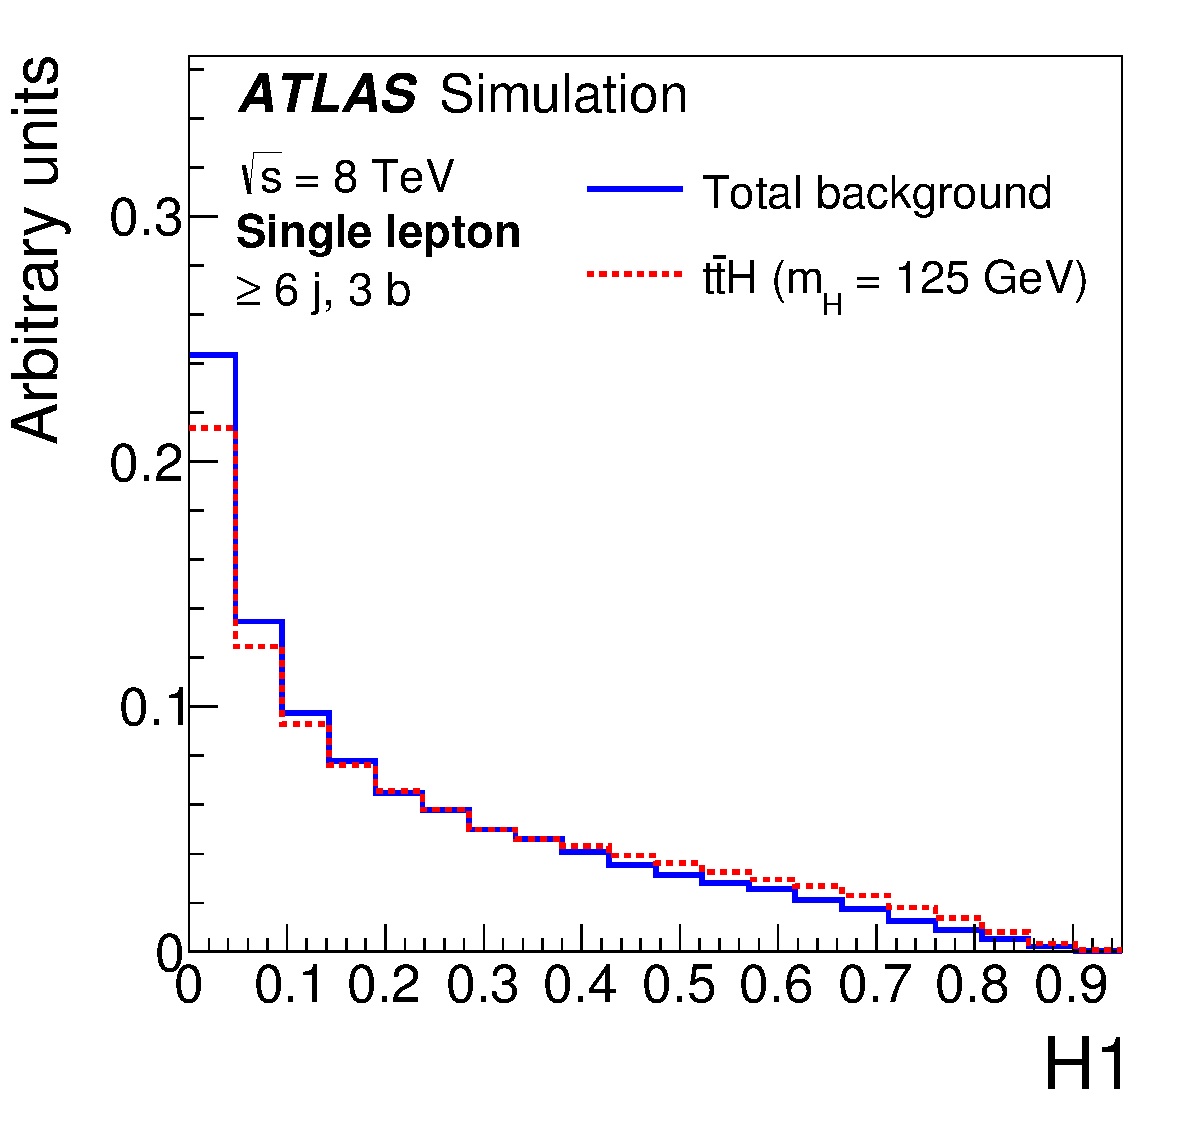
\includegraphics[width=0.49\textwidth]{Appendices/Figures_separation/H1_6jincl_sep5.pdf}
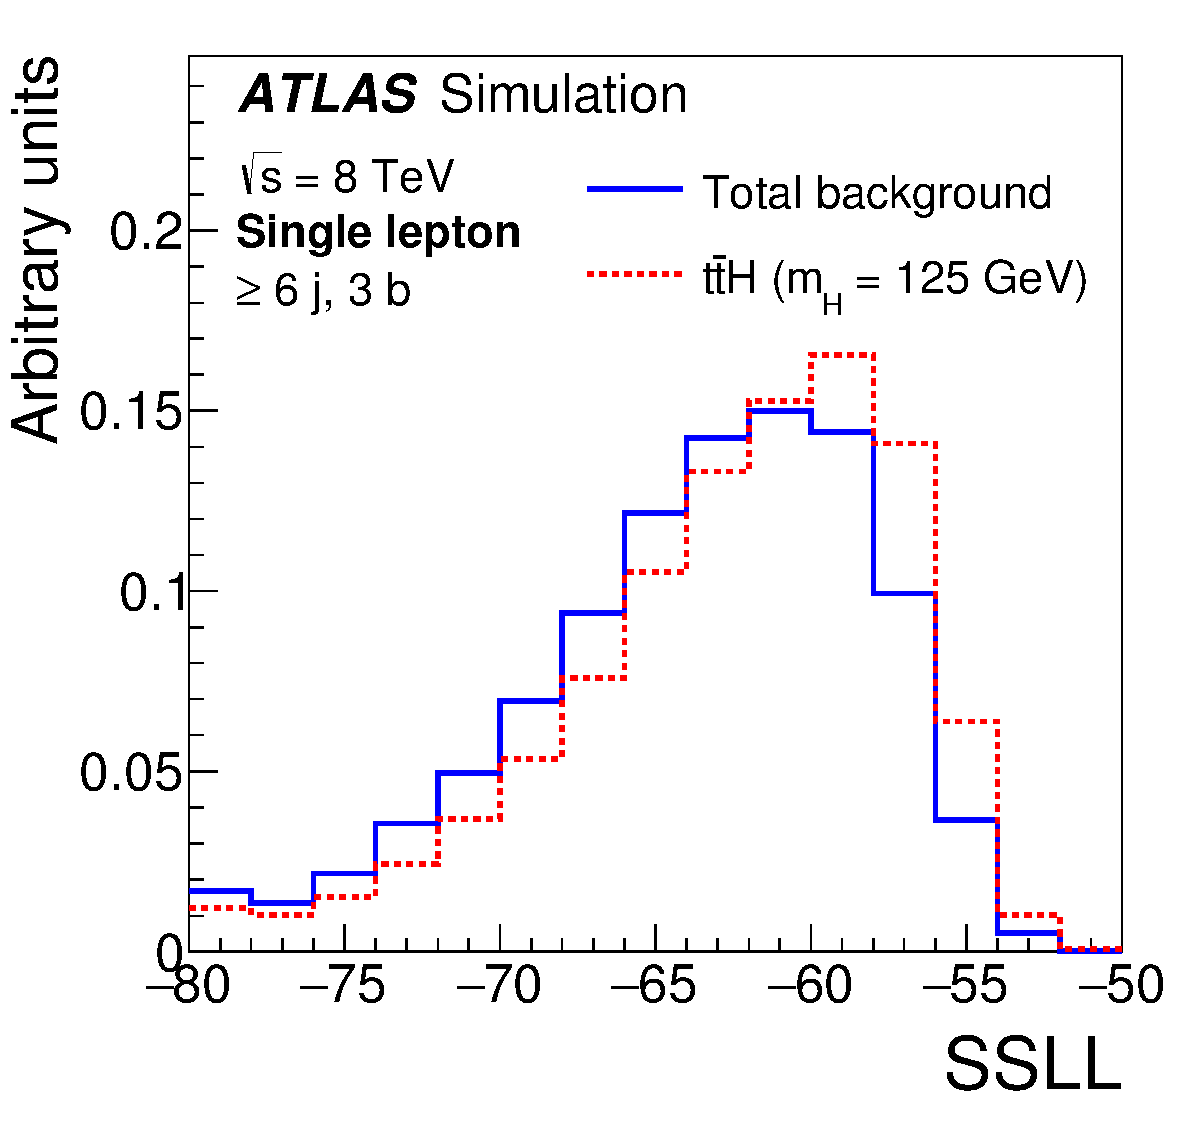
\includegraphics[width=0.49\textwidth]{Appendices/Figures_separation/ME_SLL_6jincl_sep5.pdf}
\caption{Comparison of \tth\ signal (dashed) and background (solid) for the four top-ranked input variables 
in the \sixthree\ region.  The distributions shown are (a) \numjetforty, (b) \cent, (c) $H1$, and (d) SSLL.
}
\label{fig:sepinput_lj_2} 
\end{center}
\end{figure}

\begin{figure}[tp]
\begin{center}
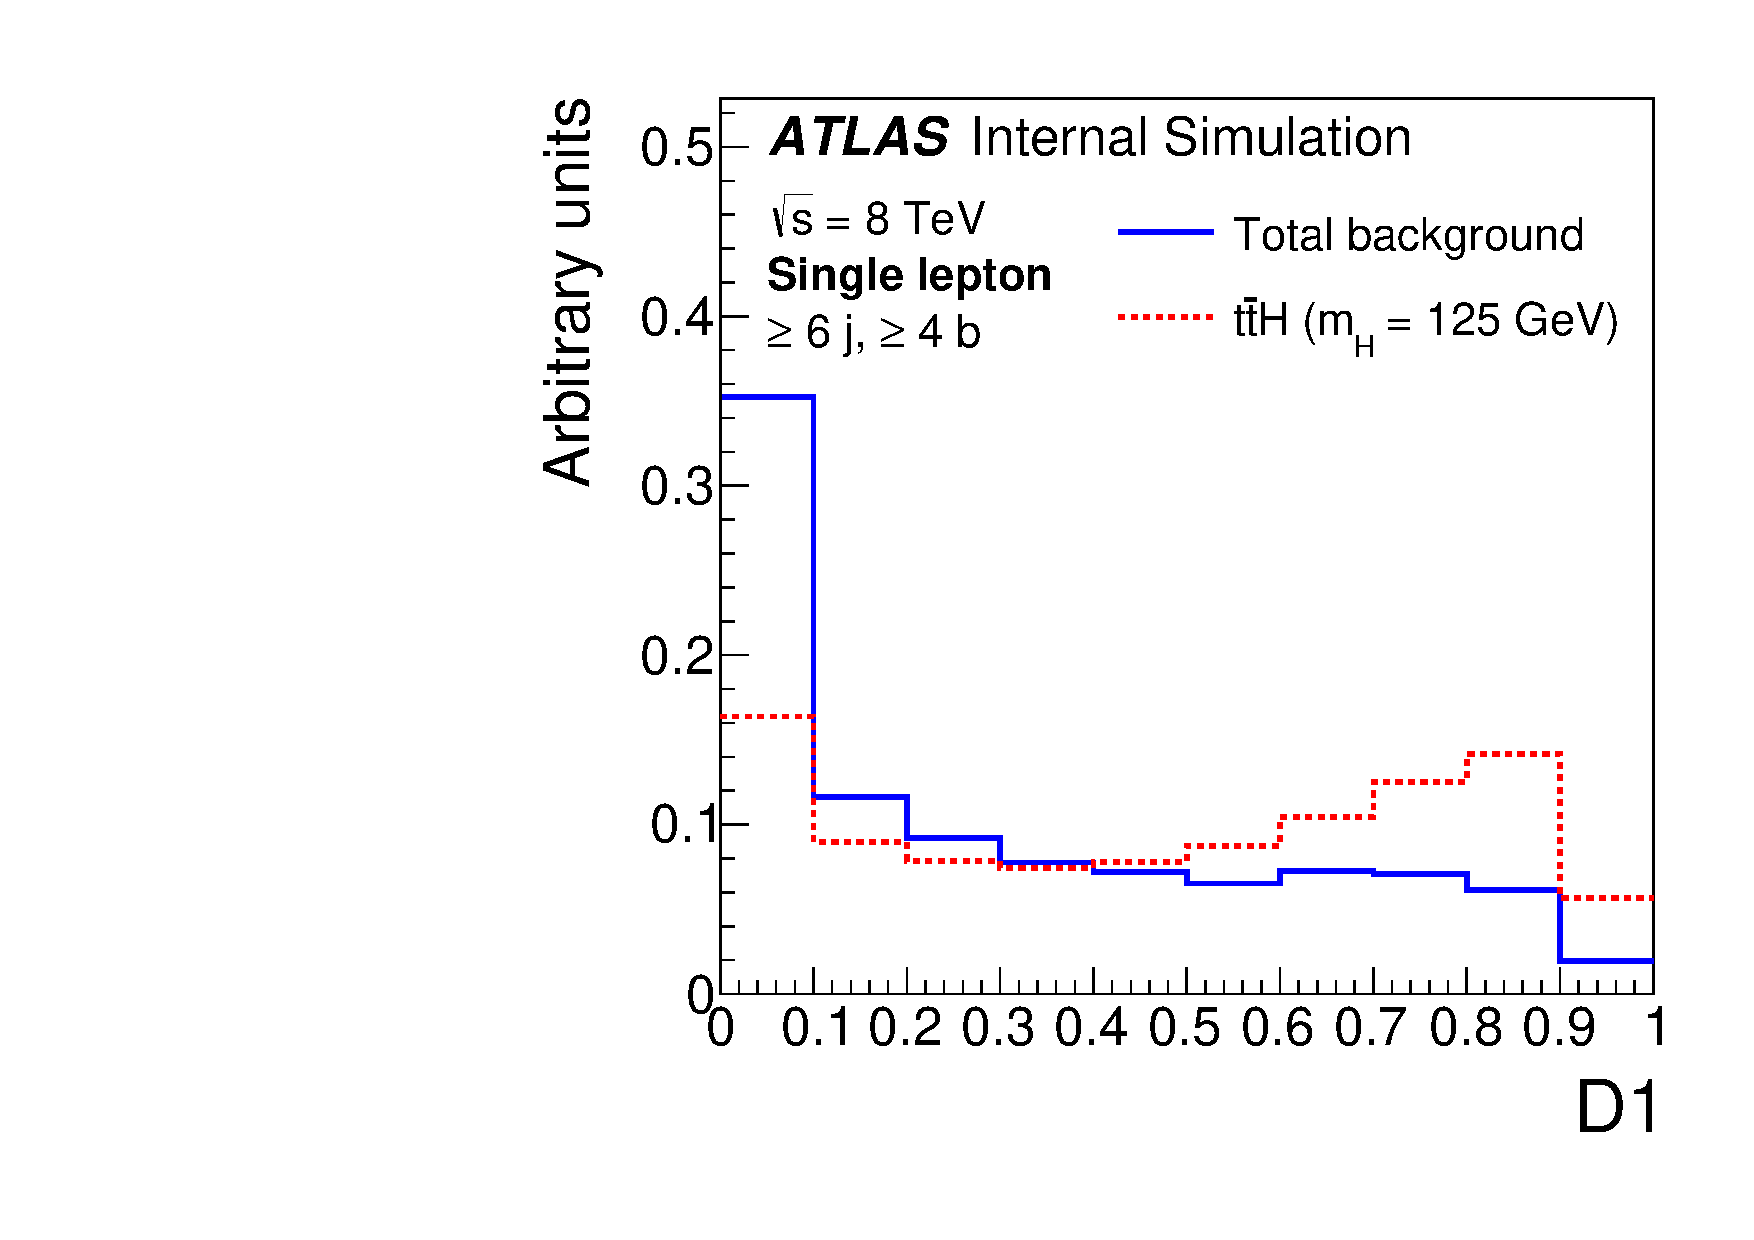
\includegraphics[width=0.49\textwidth]{Appendices/Figures_separation/ME_D1_6jincl_sep.pdf}
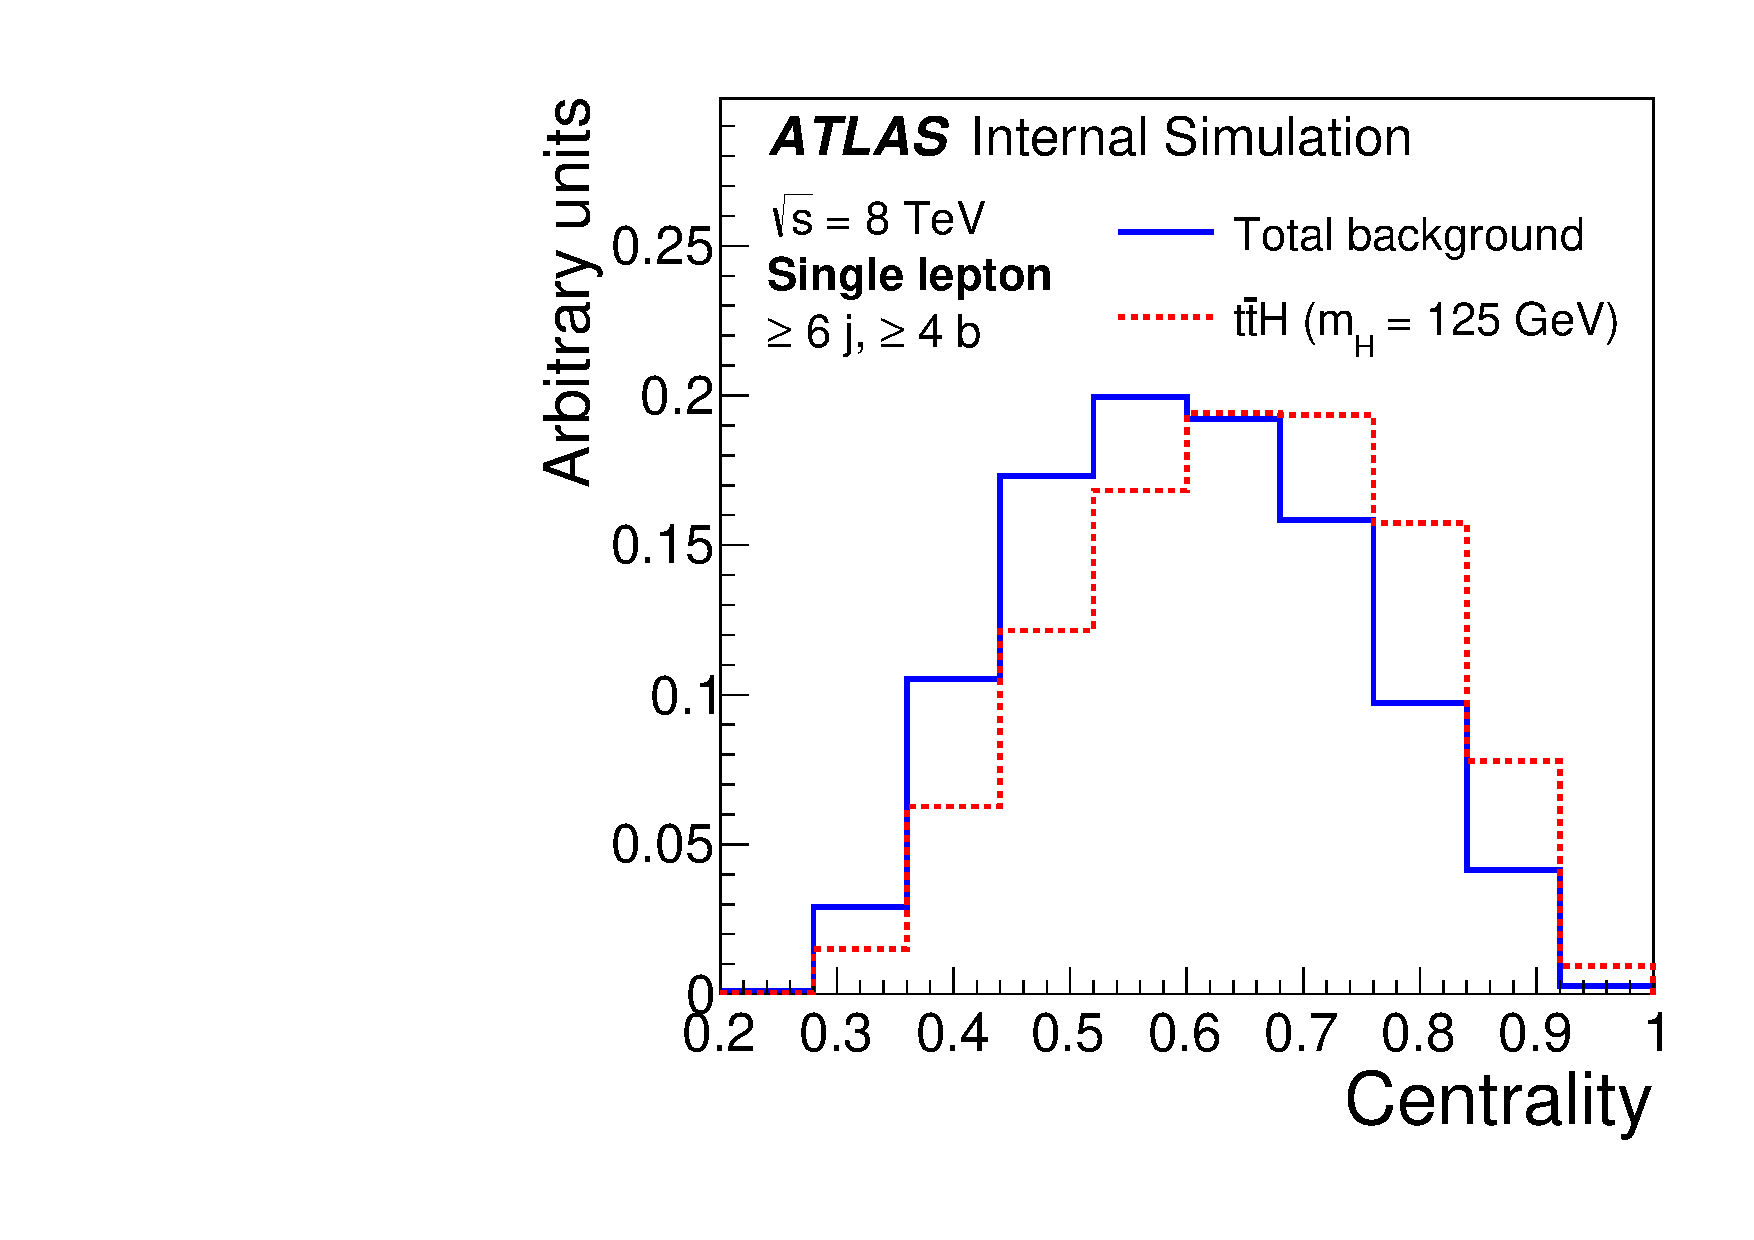
\includegraphics[width=0.49\textwidth]{Appendices/Figures_separation/cent_6jincl_sep.pdf}\\
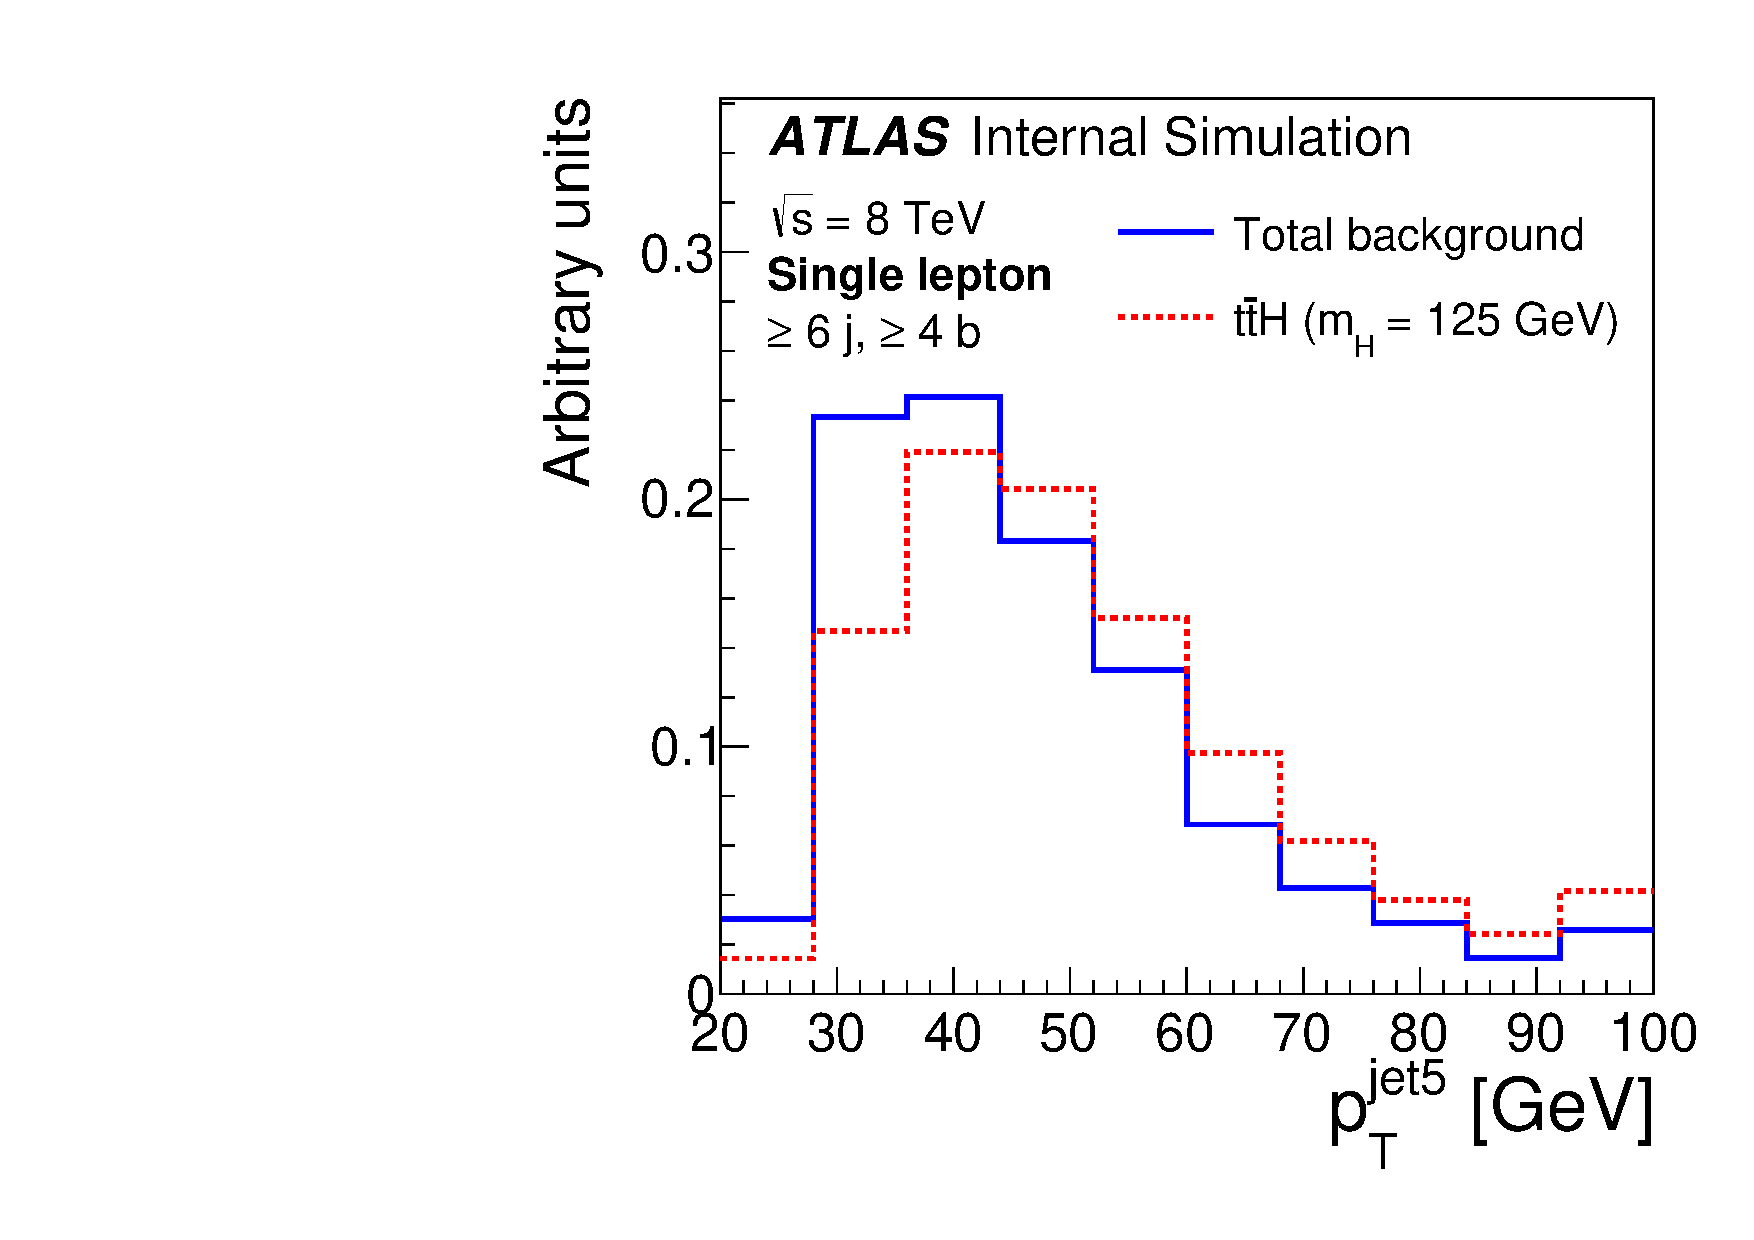
\includegraphics[width=0.49\textwidth]{Appendices/Figures_separation/jet5_pt_6jincl_sep.pdf}
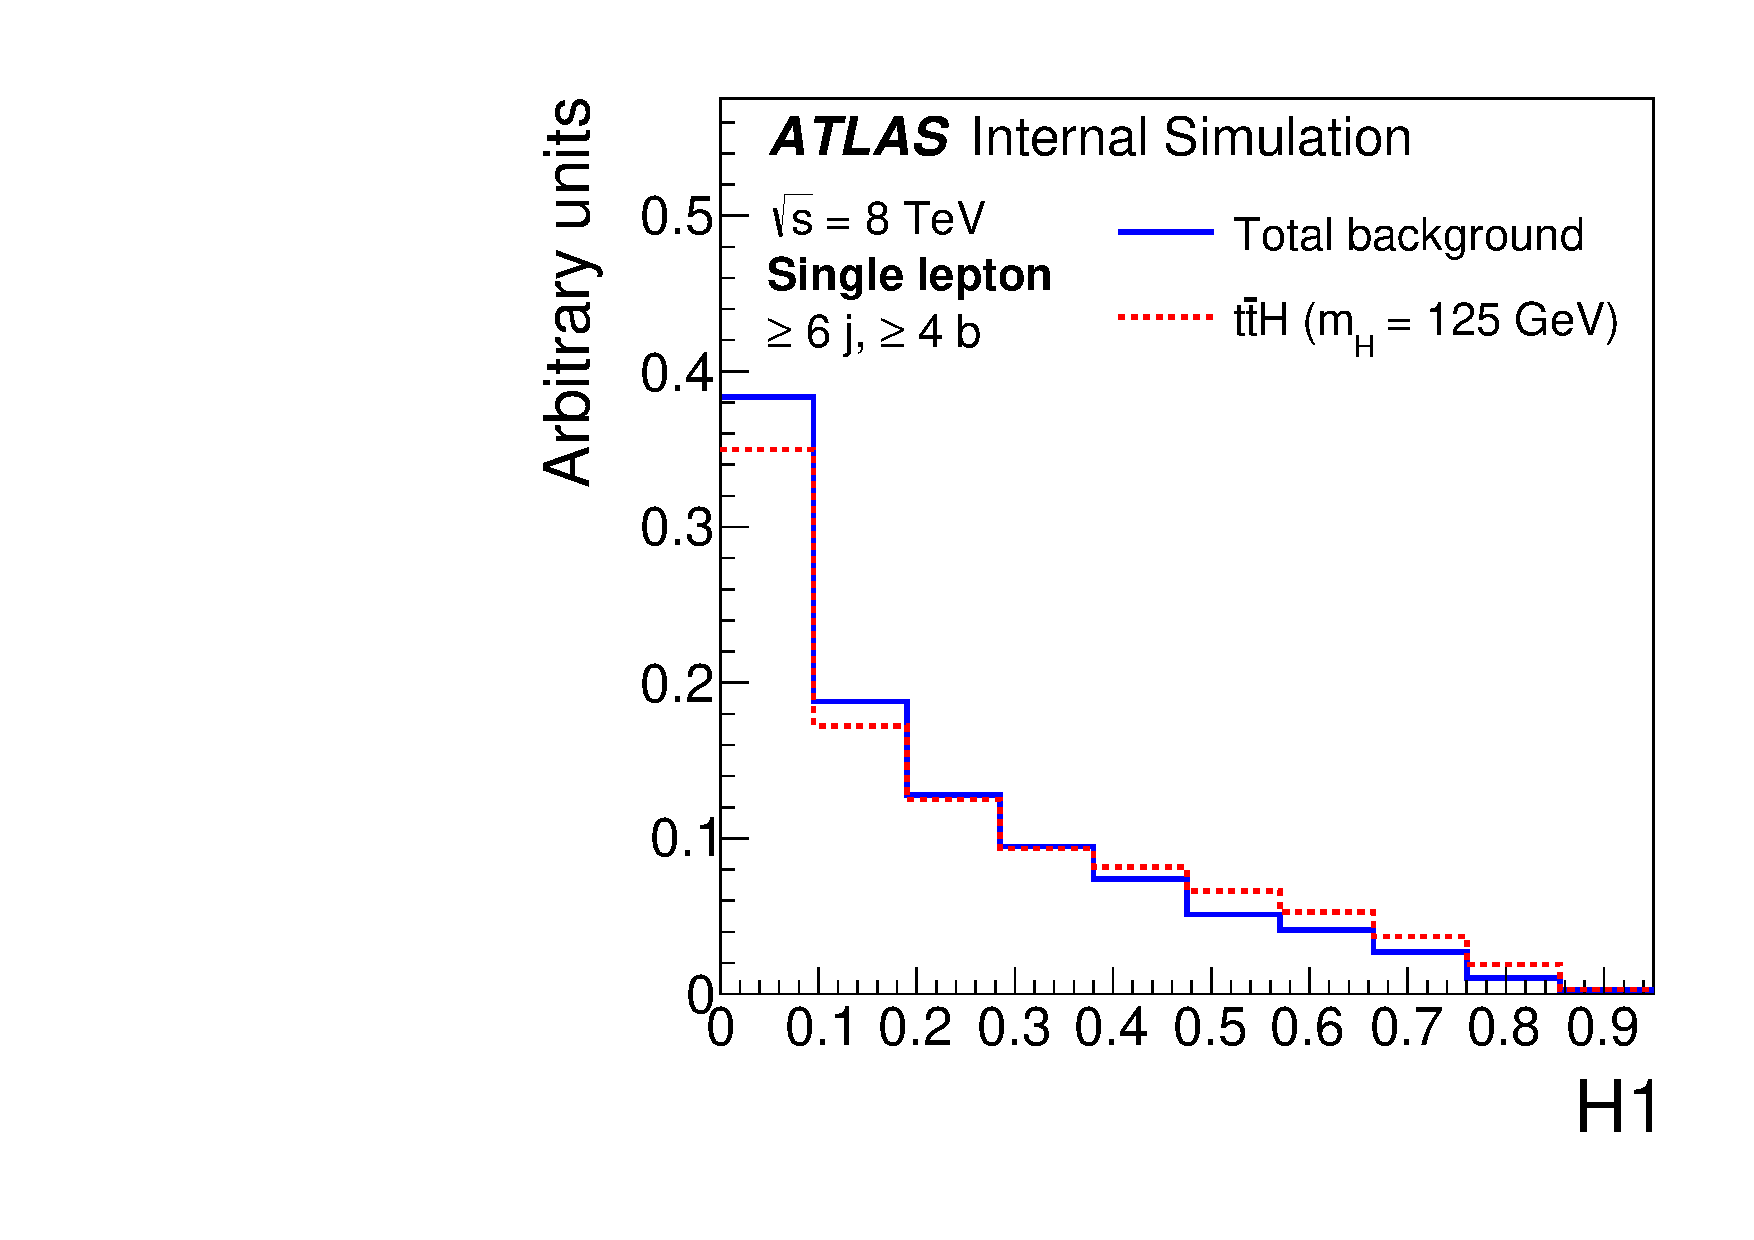
\includegraphics[width=0.49\textwidth]{Appendices/Figures_separation/H1_6jincl_sep.pdf}
\caption{Comparison of \tth\ signal (dashed) and background (solid) for the four top-ranked input variables 
in the \sixfour\ region.  The distributions shown are (a) $D1$, (b) \cent, (c) \ptjetfive, and (d) $H1$.
}
\label{fig:sepinput_lj_3} 
\end{center}
\end{figure}

\clearpage

\begin{figure}[tp]
\begin{center}
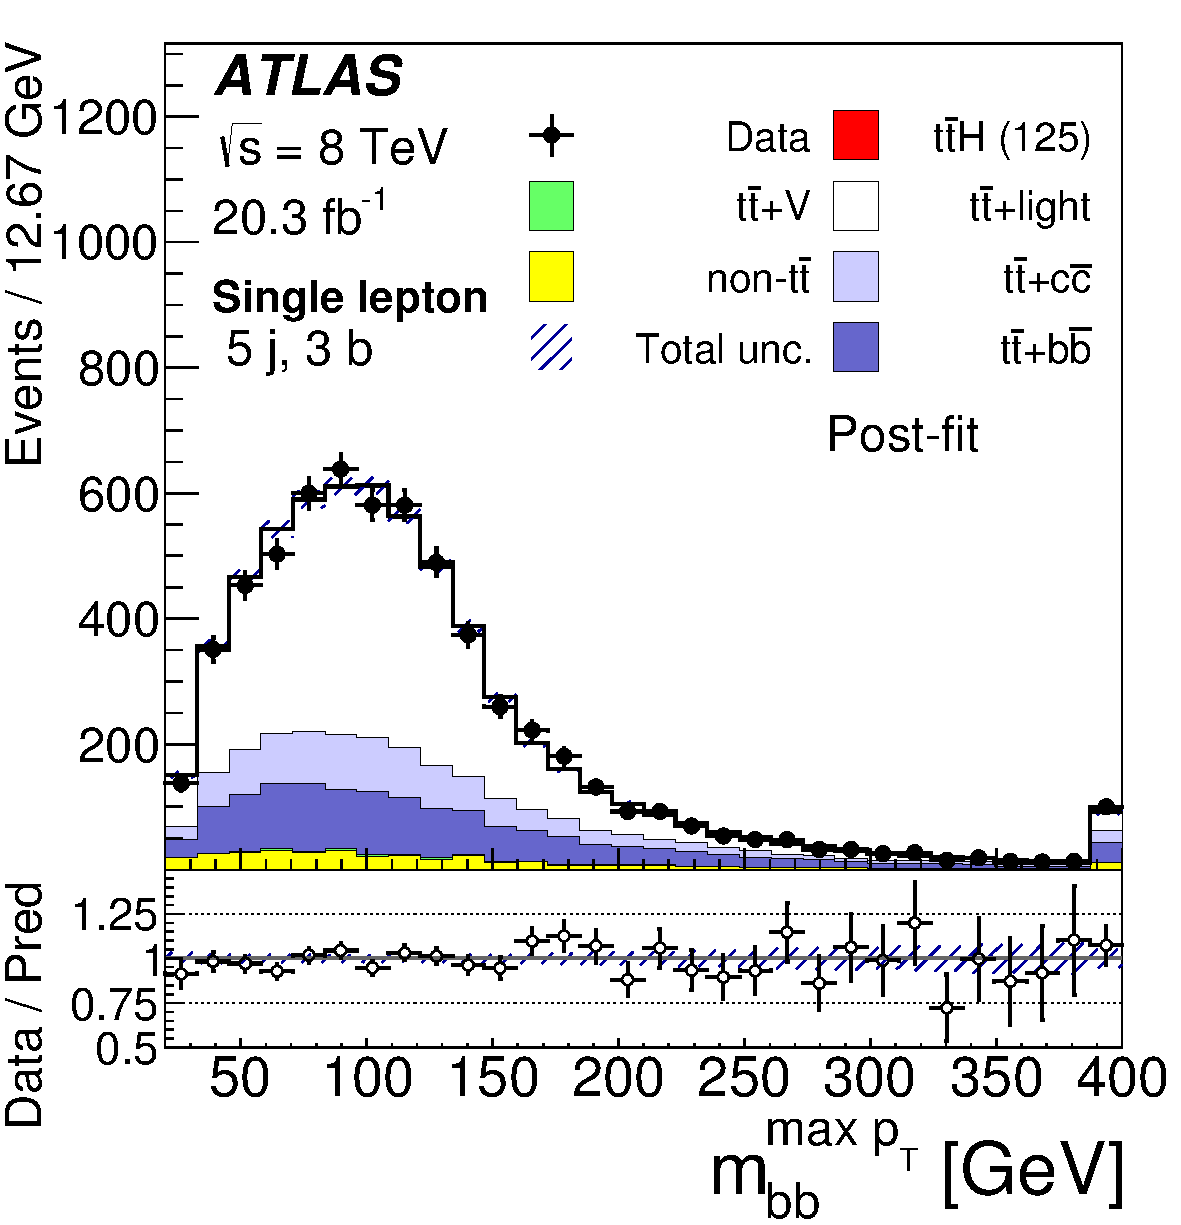
\includegraphics[width=0.49\textwidth]{Appendices/Figures_separation/mbb_maxPt_flav_5.pdf}
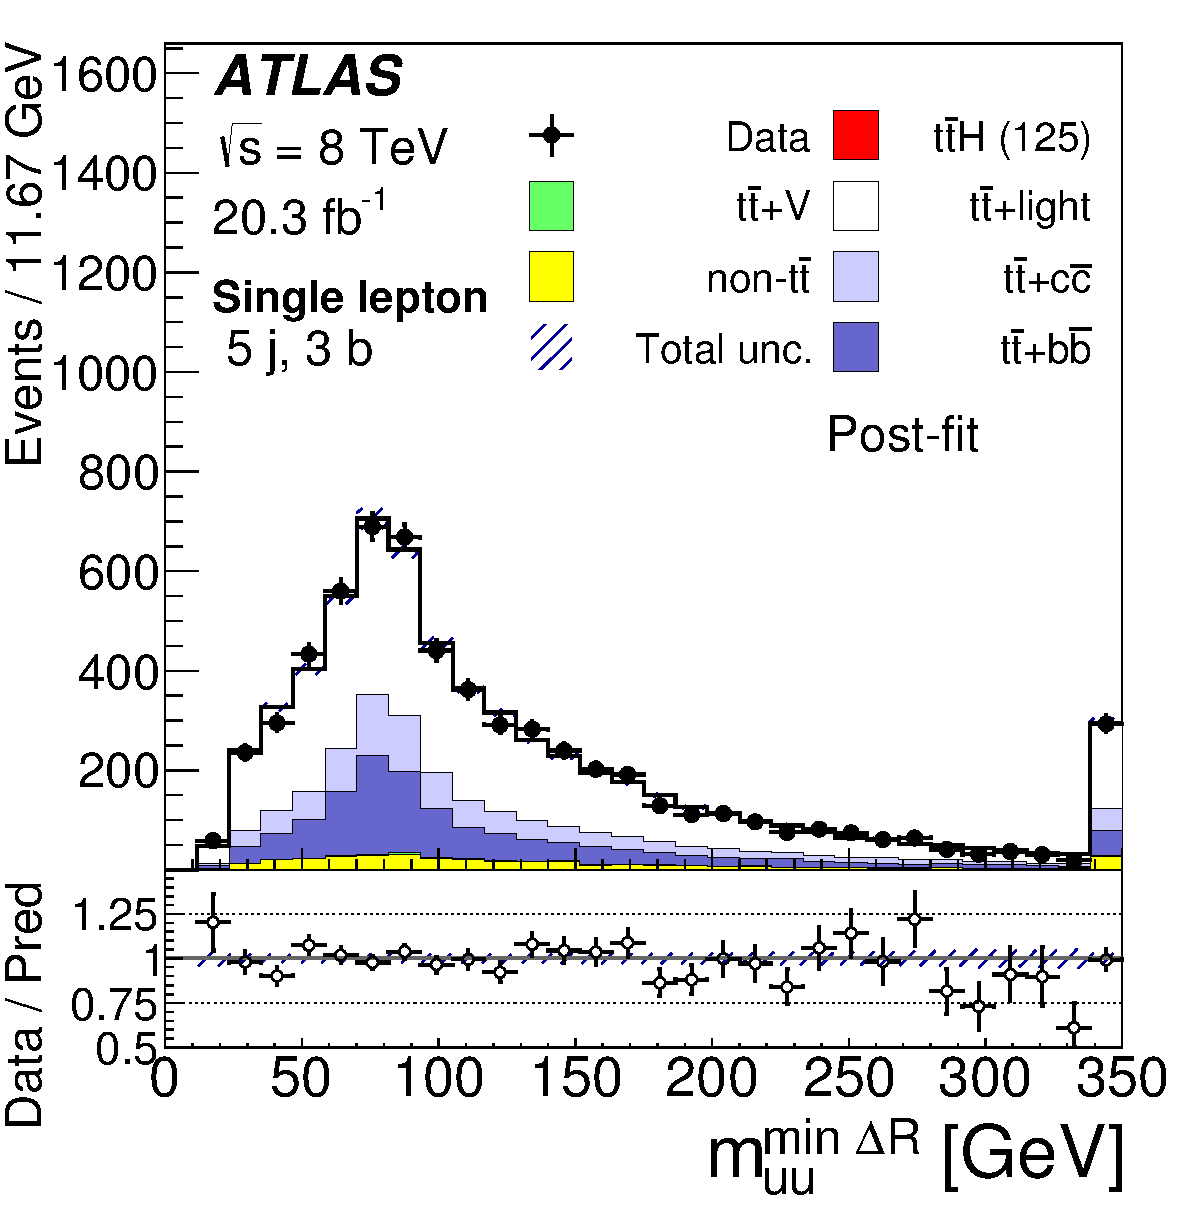
\includegraphics[width=0.49\textwidth]{Appendices/Figures_separation/WhadM_flav_5.pdf} \\
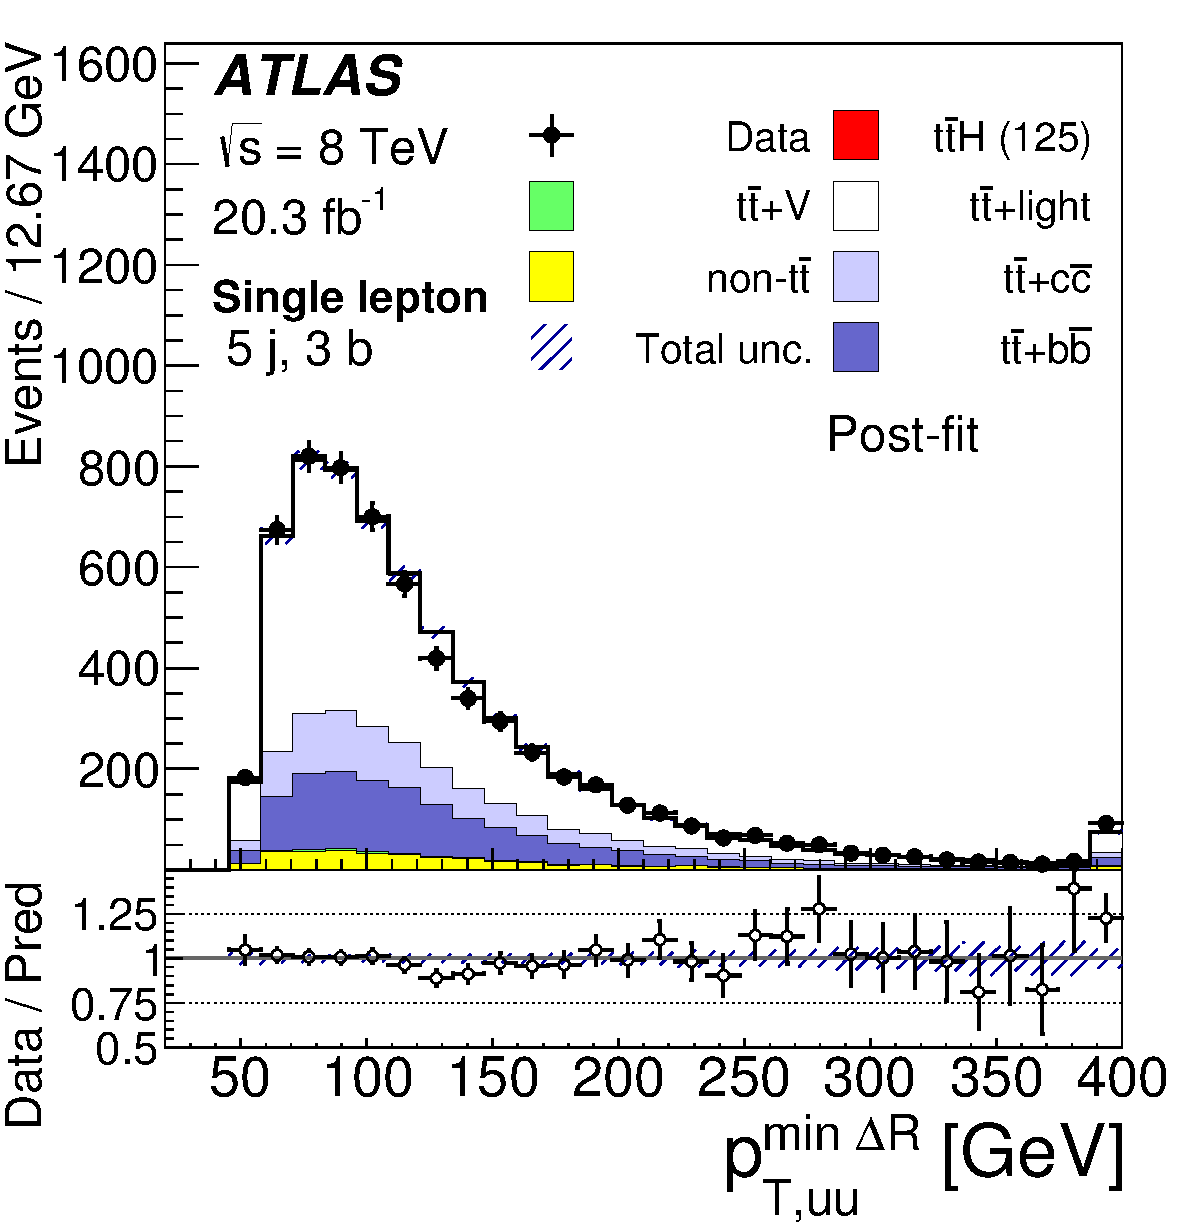
\includegraphics[width=0.49\textwidth]{Appendices/Figures_separation/WhadSpt_flav_5.pdf}
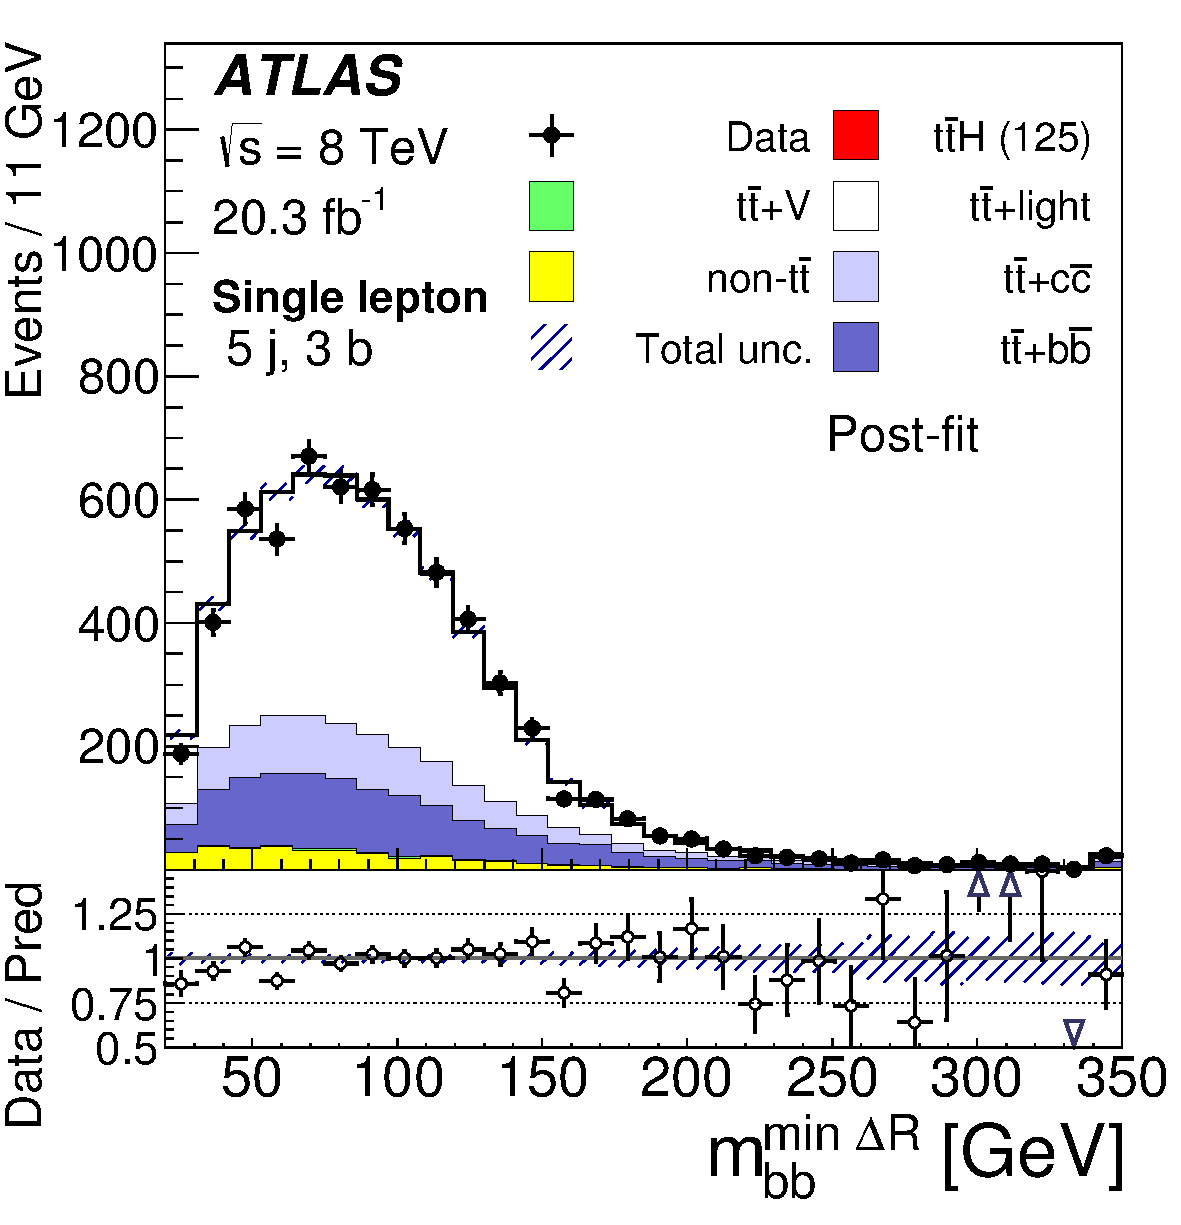
\includegraphics[width=0.49\textwidth]{Appendices/Figures_separation/mbb_mindR_flav_5.pdf}
\caption{Post-fit comparison of data and prediction for the four top-ranked input variables in the 
\fivethree\ region. The distributions shown are (a) \mbbmaxpt, (b) \whadmass, (c)  \whadpt and (d) \mbbmindr.
The first and last bins in all figures contain the underflow and 
overflow, respectively. The bottom panel displays the ratio of 
data to the total prediction. The hashed area represents the uncertainty on the background. }
\label{fig:postinput_lj_0} 
\end{center}
\end{figure}

\begin{figure}[tp]
\begin{center}
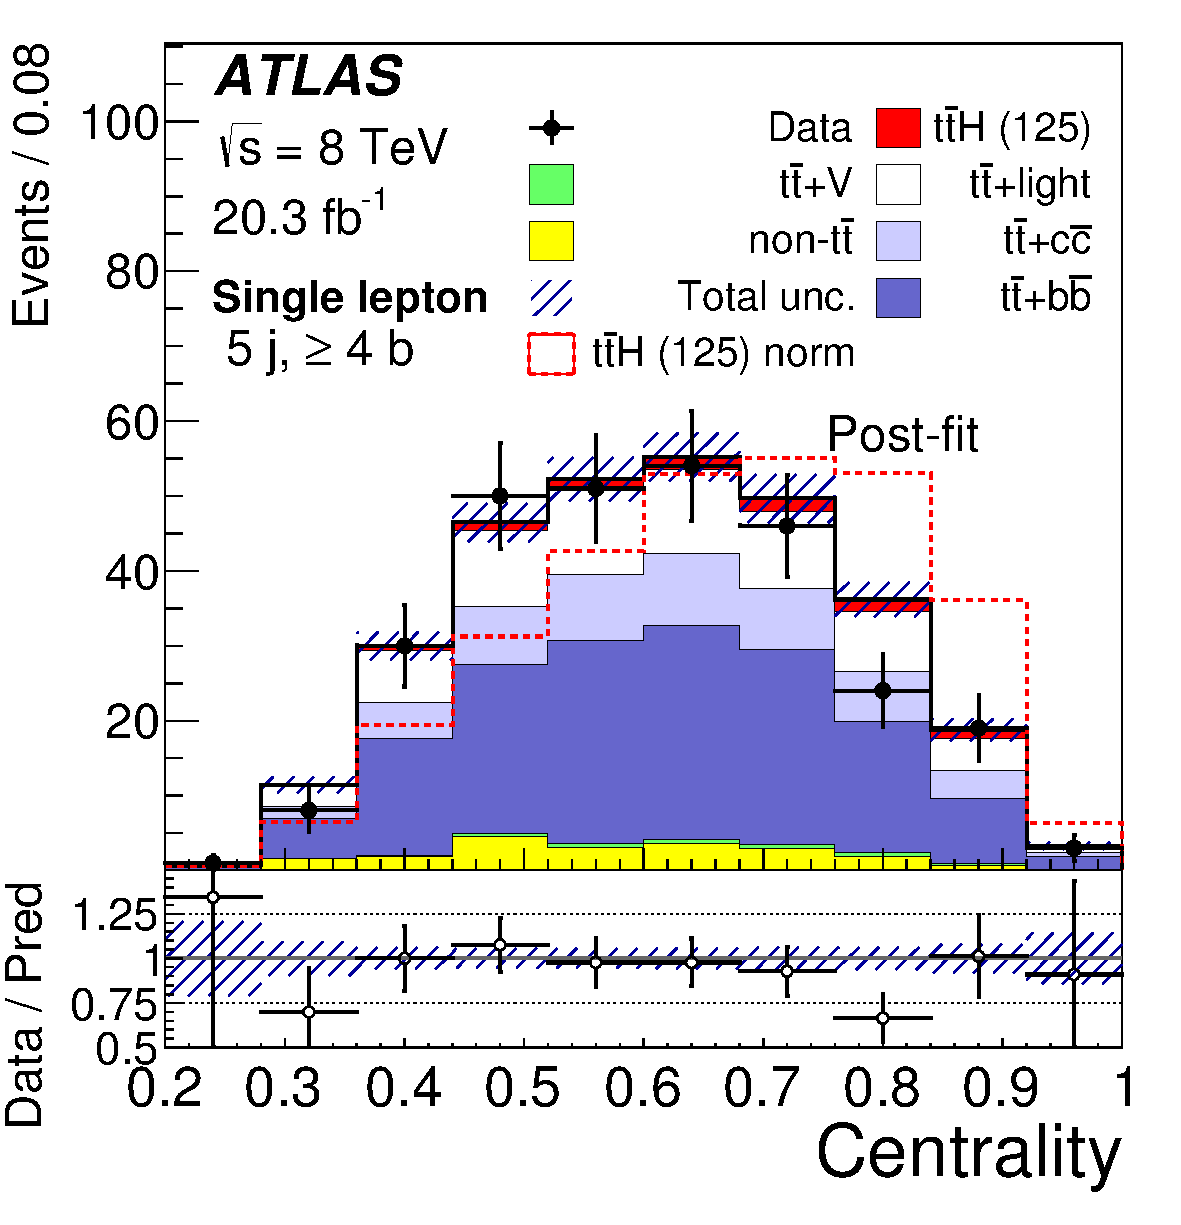
\includegraphics[width=0.49\textwidth]{Appendices/Figures_separation/cent_5.pdf}
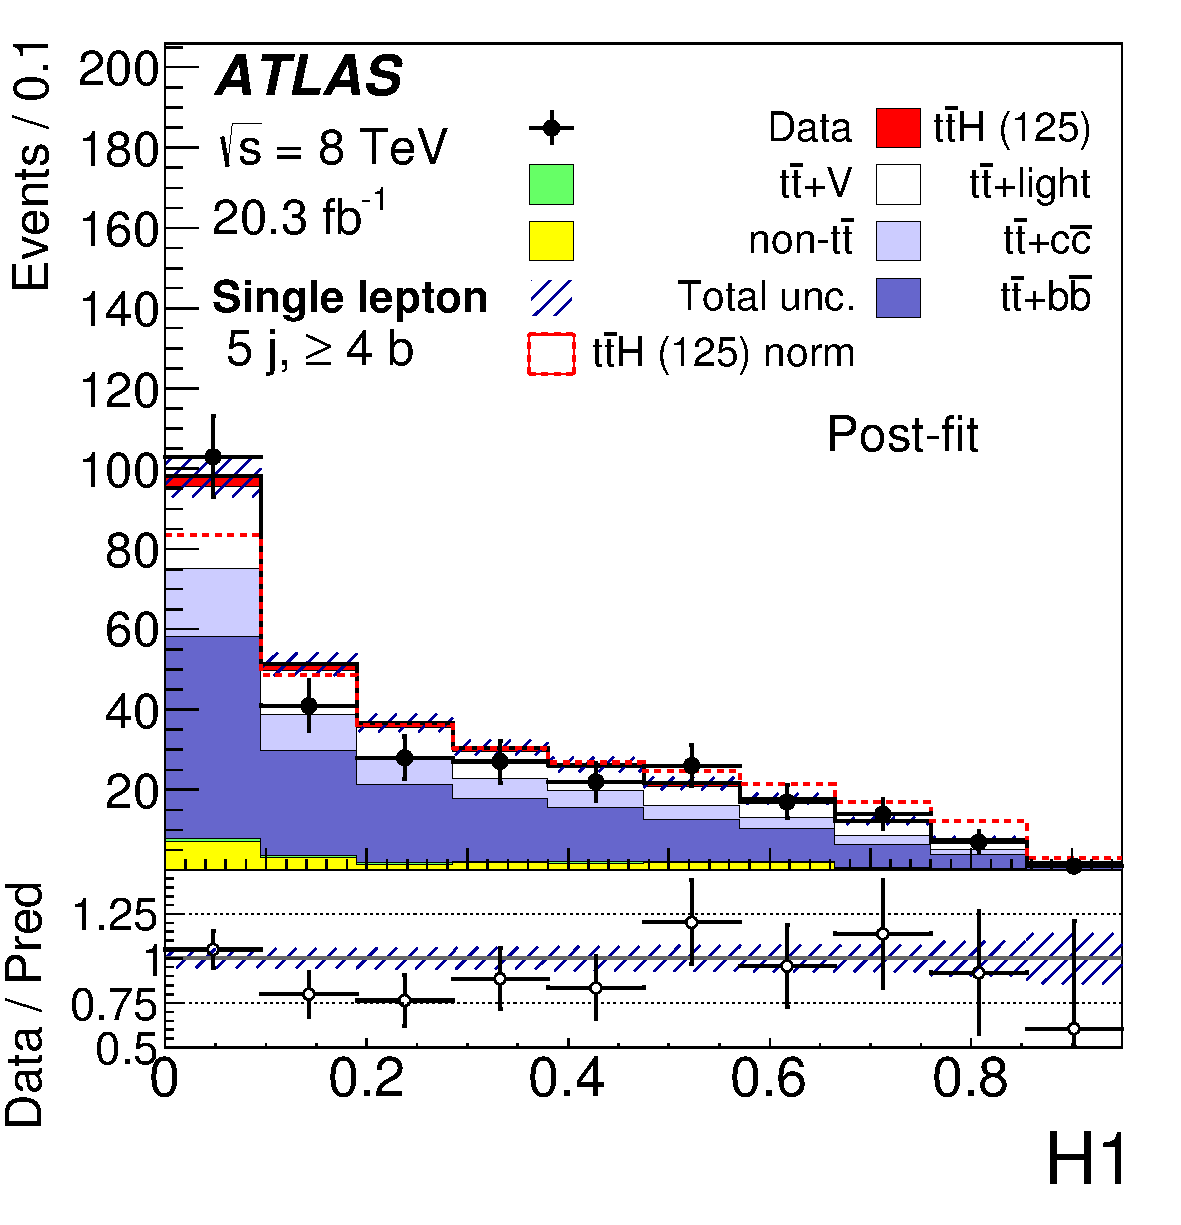
\includegraphics[width=0.49\textwidth]{Appendices/Figures_separation/H1_5.pdf}\\
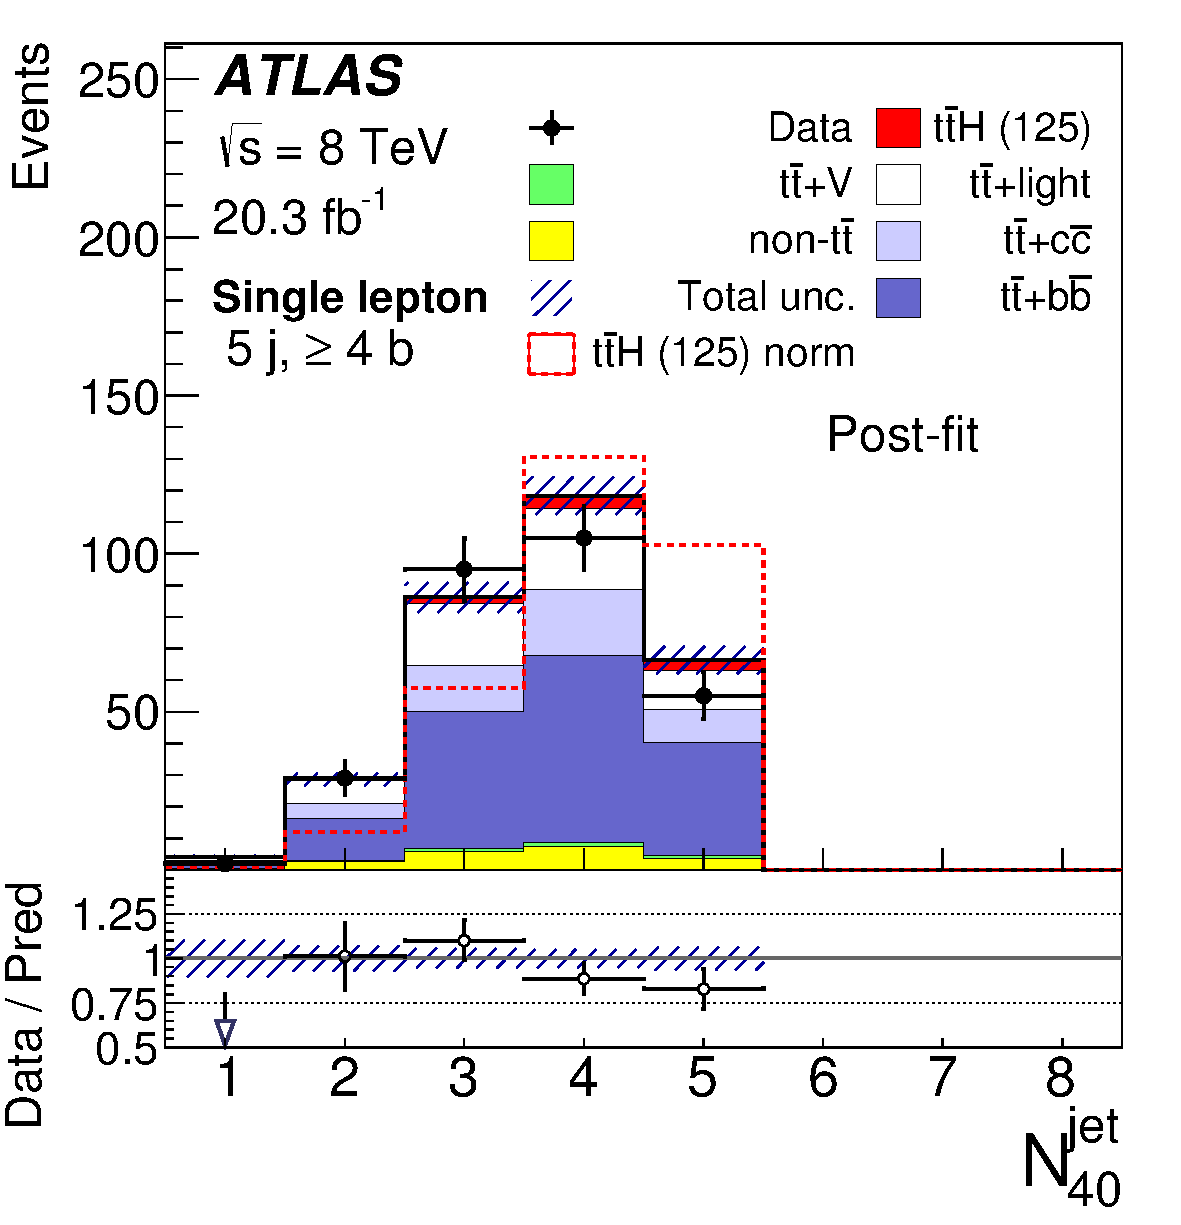
\includegraphics[width=0.49\textwidth]{Appendices/Figures_separation/num_jet_40_5.pdf}
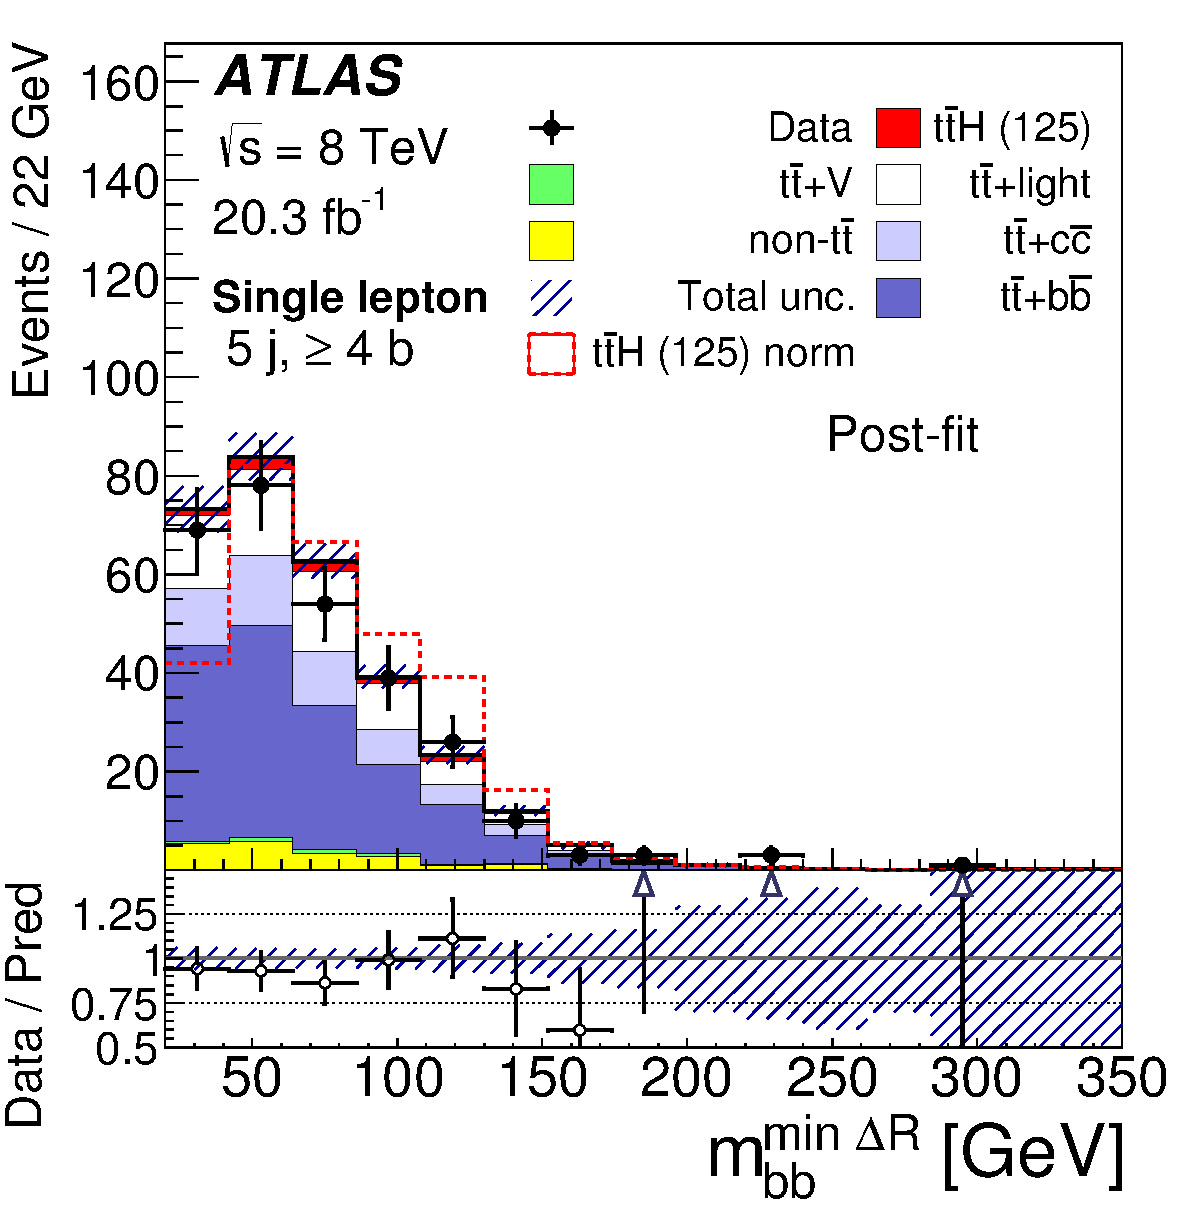
\includegraphics[width=0.49\textwidth]{Appendices/Figures_separation/mbb_mindR_5.pdf}
\caption{Post-fit comparison of data and prediction for the four top-ranked input variables in the 
\fivefour\ region. The distributions shown are (a) \cent, (b) $H1$, (c)  \numjetforty and (d) \mbbmindr.
The first and last bins in all figures contain the underflow and
overflow, respectively. The bottom panel displays the ratio of 
data to the total prediction. The hashed area represents the uncertainty on the background.
The dashed line shows \tth\ signal
distribution normalized to background yield. The \tth\ signal yield (solid) 
is normalized to the fitted $\mu$.}
\label{fig:postinput_lj_1} 
\end{center}
\end{figure}

\begin{figure}[tp]
\begin{center}
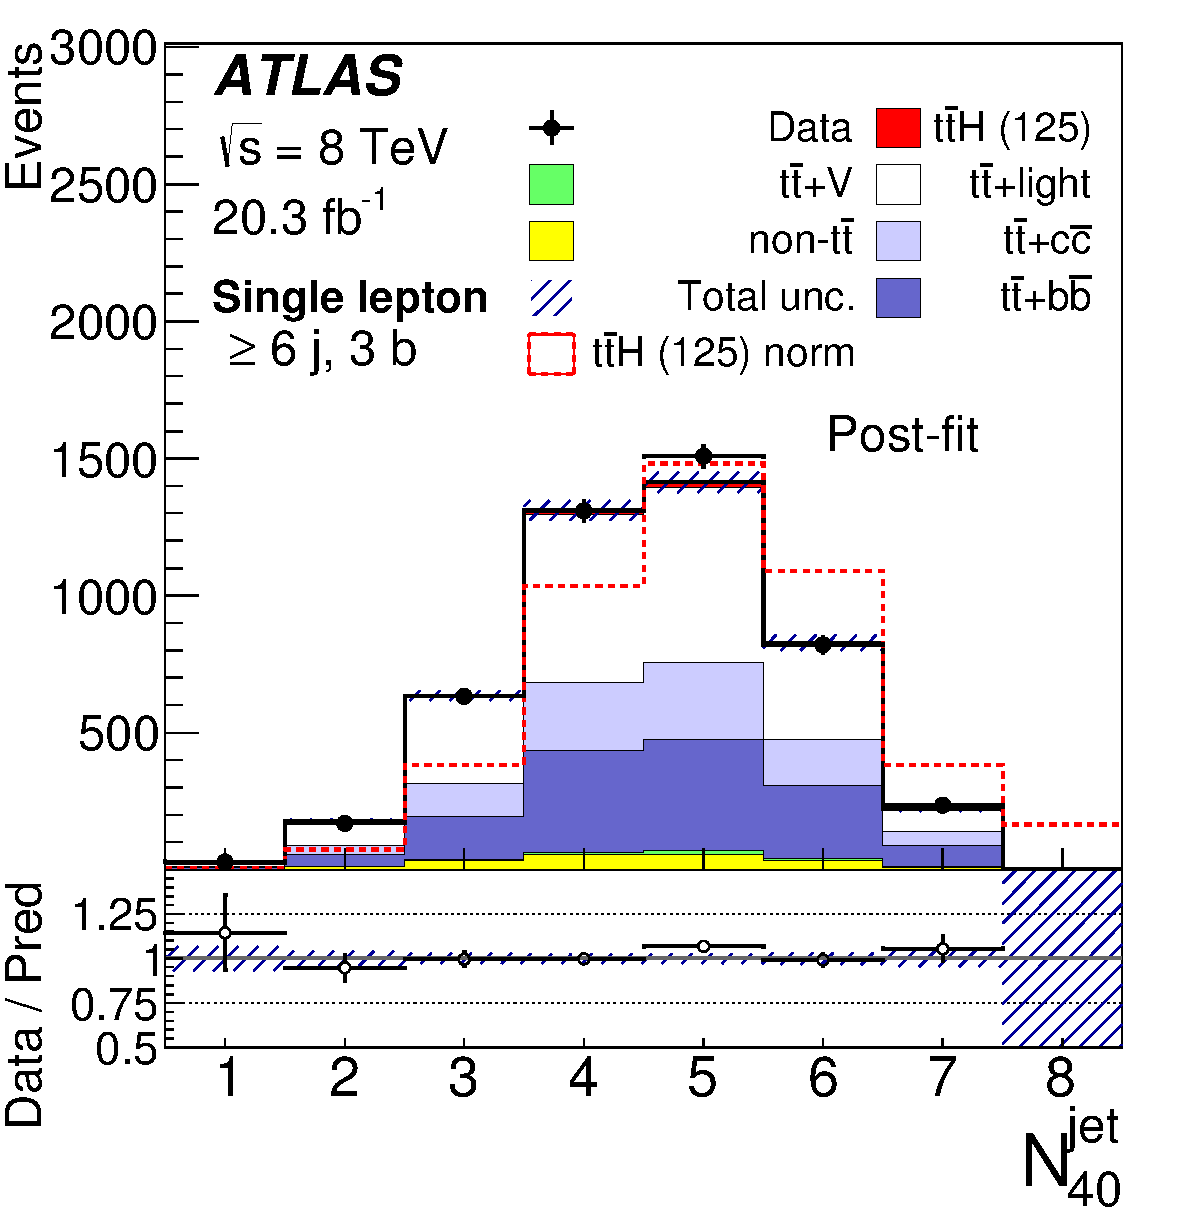
\includegraphics[width=0.49\textwidth]{Appendices/Figures_separation/num_jet_40_6jincl5.pdf}
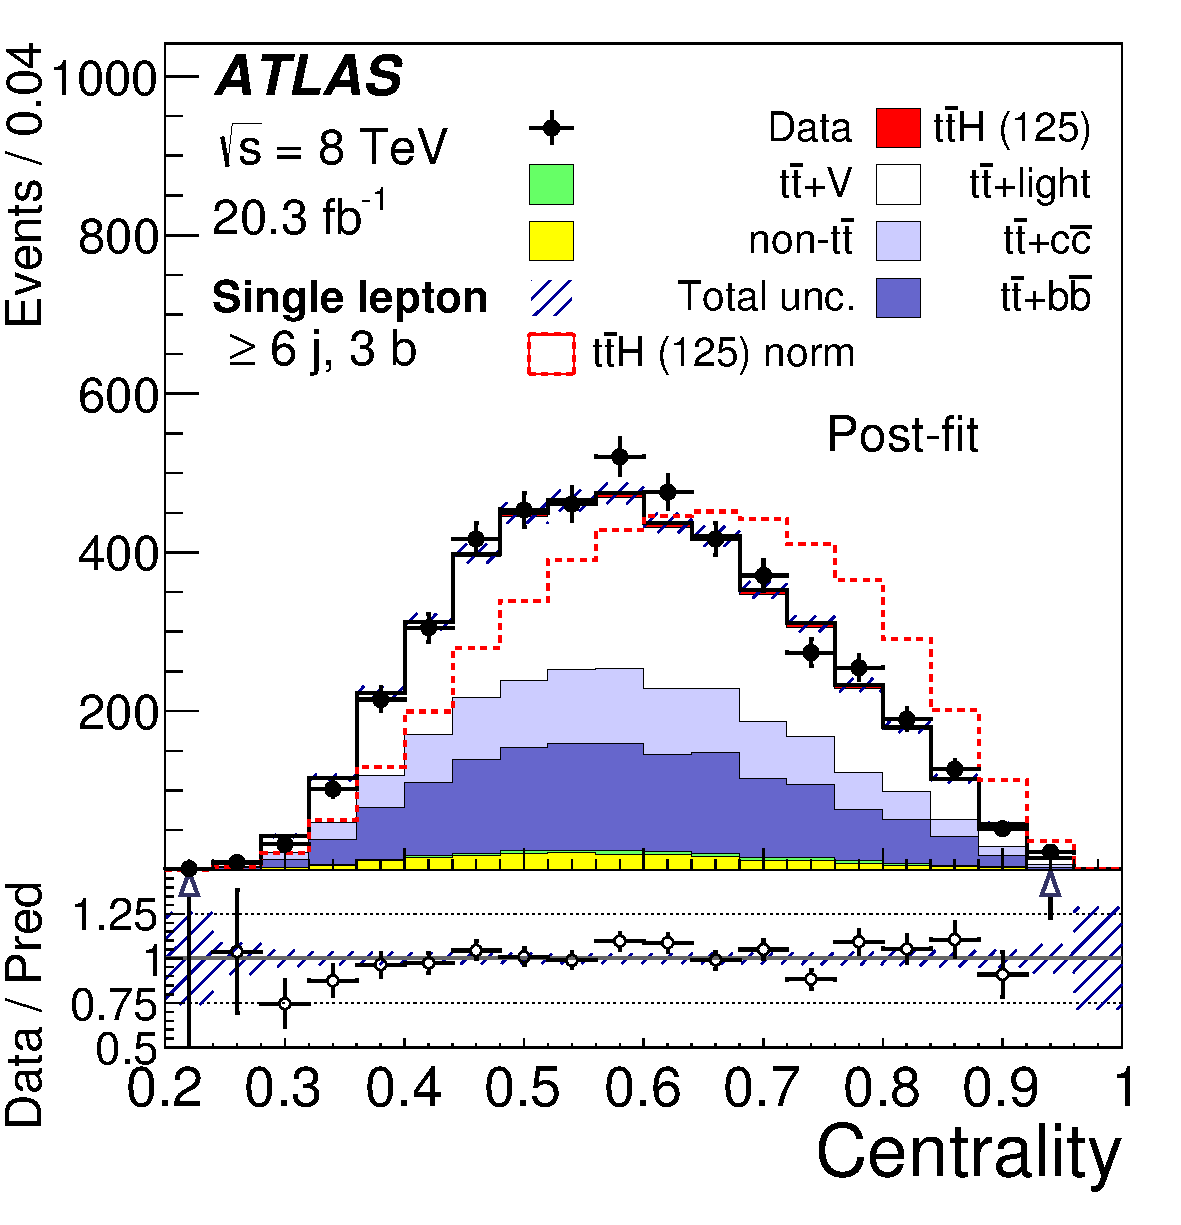
\includegraphics[width=0.49\textwidth]{Appendices/Figures_separation/cent_6jincl5.pdf} \\
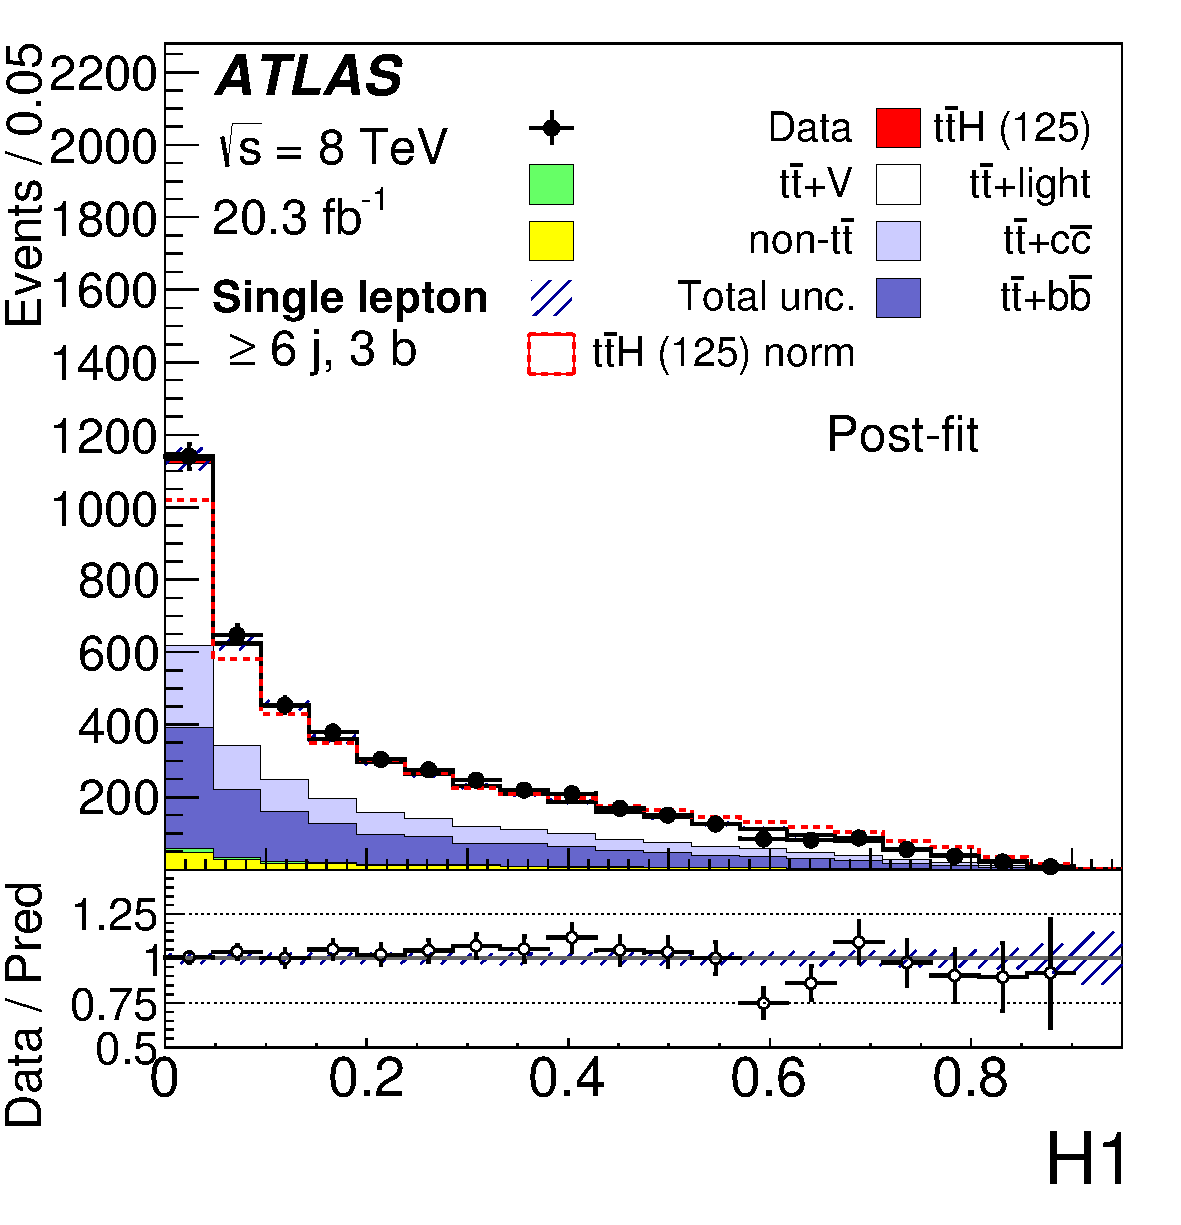
\includegraphics[width=0.49\textwidth]{Appendices/Figures_separation/H1_6jincl5.pdf}
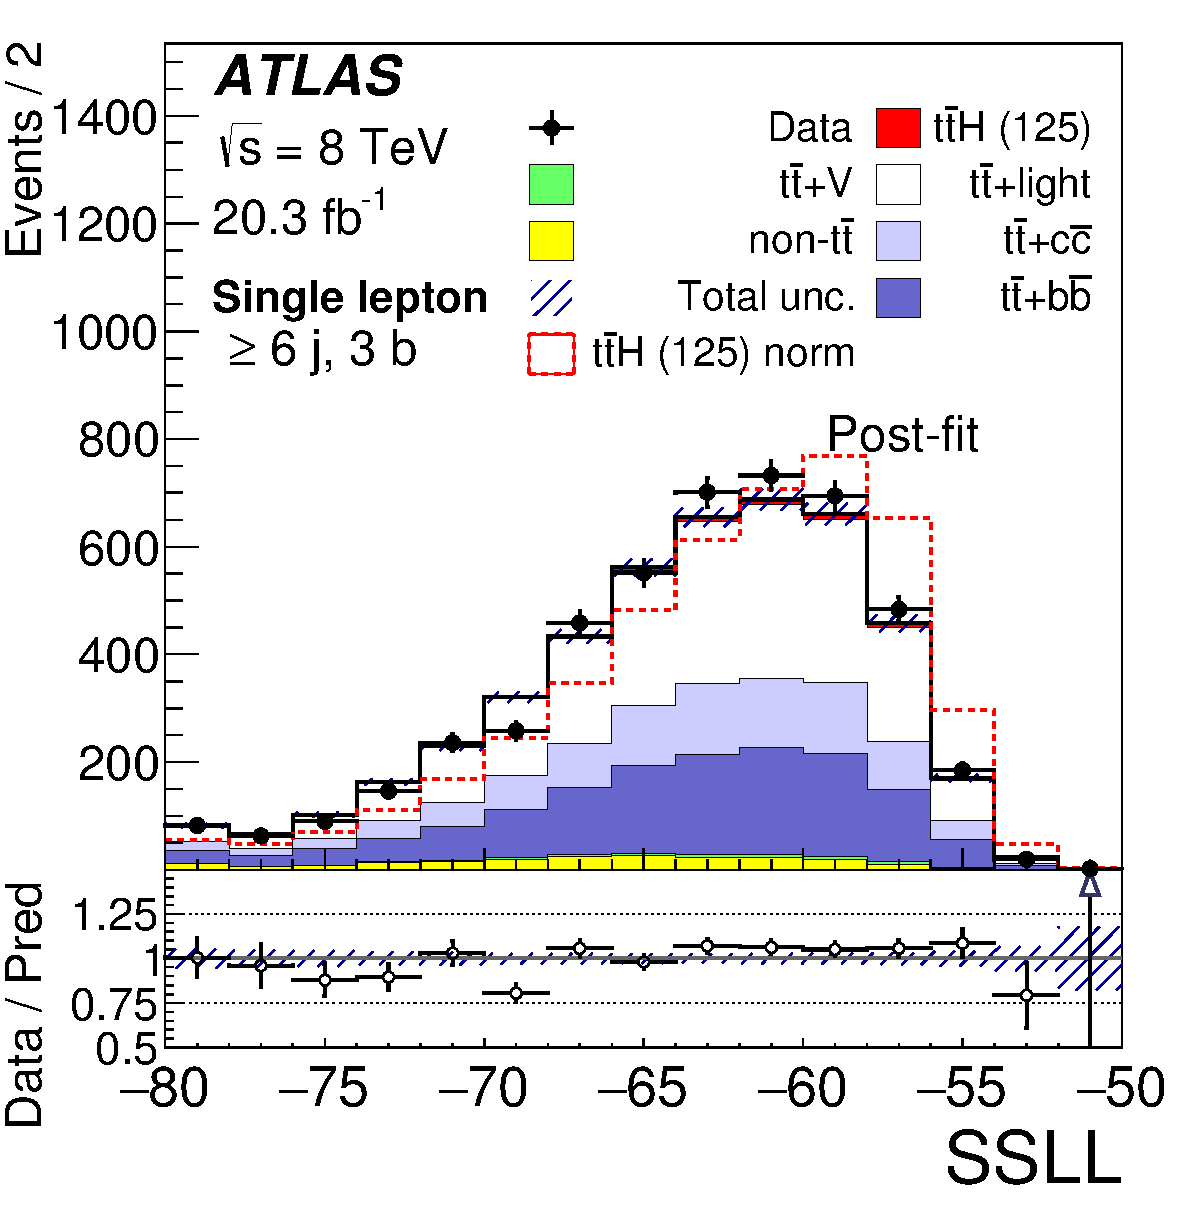
\includegraphics[width=0.49\textwidth]{Appendices/Figures_separation/ME_SLL_6jincl5.pdf}
\caption{Post-fit comparison of data and prediction for the four top-ranked input variables in 
\sixthree\ region. The distributions shown are (a) \numjetforty, (b) \cent, (c) $H1$, 
and (d) SSLL.
The first and last bins in all figures contain the underflow and
overflow, respectively. The bottom panel displays the ratio of 
data to the total prediction. The hashed area represents the uncertainty on the background.
The dashed line shows \tth\ signal
distribution normalized to background yield. The \tth\ signal yield (solid) 
is normalized to the fitted $\mu$.}
\label{fig:postinput_lj_2} 
\end{center}
\end{figure}

\begin{figure}[tp]
\begin{center}
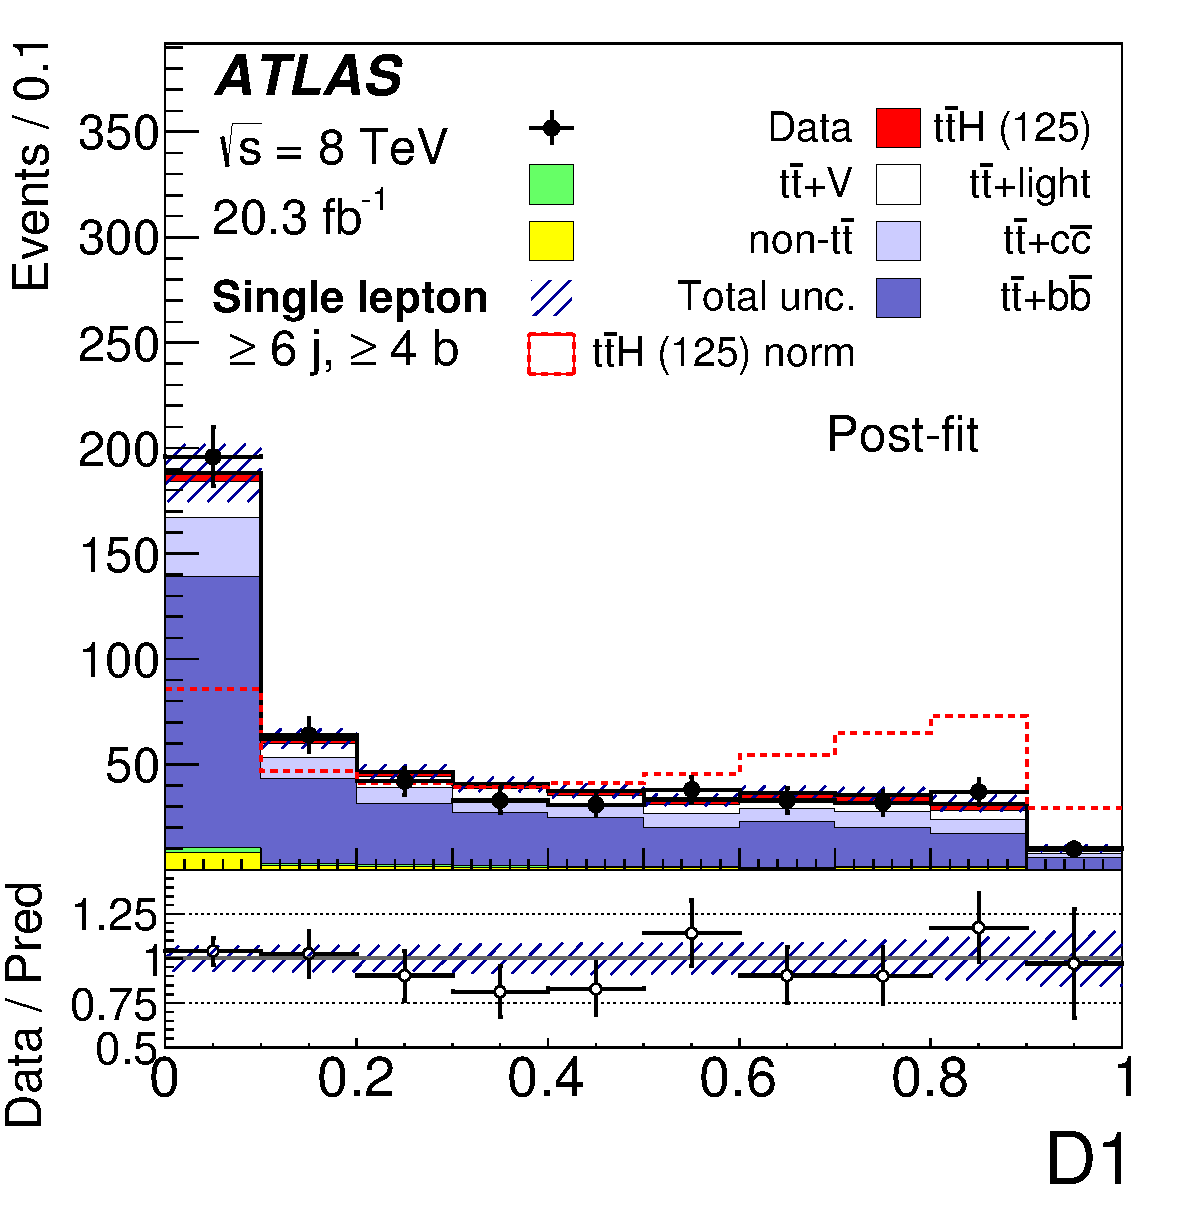
\includegraphics[width=0.49\textwidth]{Appendices/Figures_separation/ME_D1_6jincl.pdf}
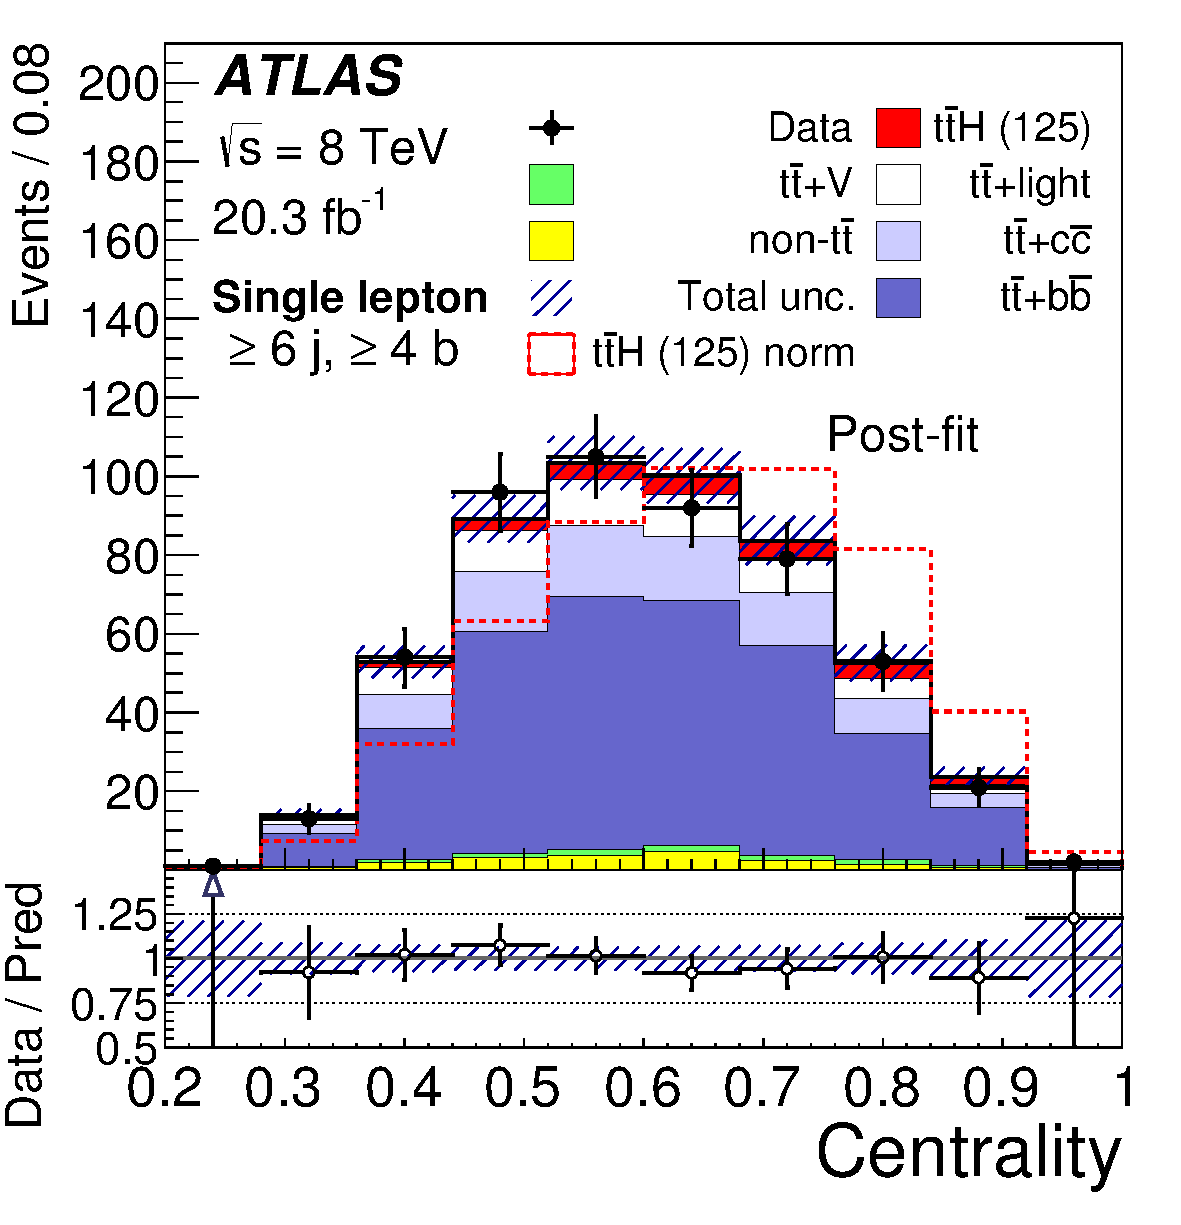
\includegraphics[width=0.49\textwidth]{Appendices/Figures_separation/cent_6jincl.pdf} \\
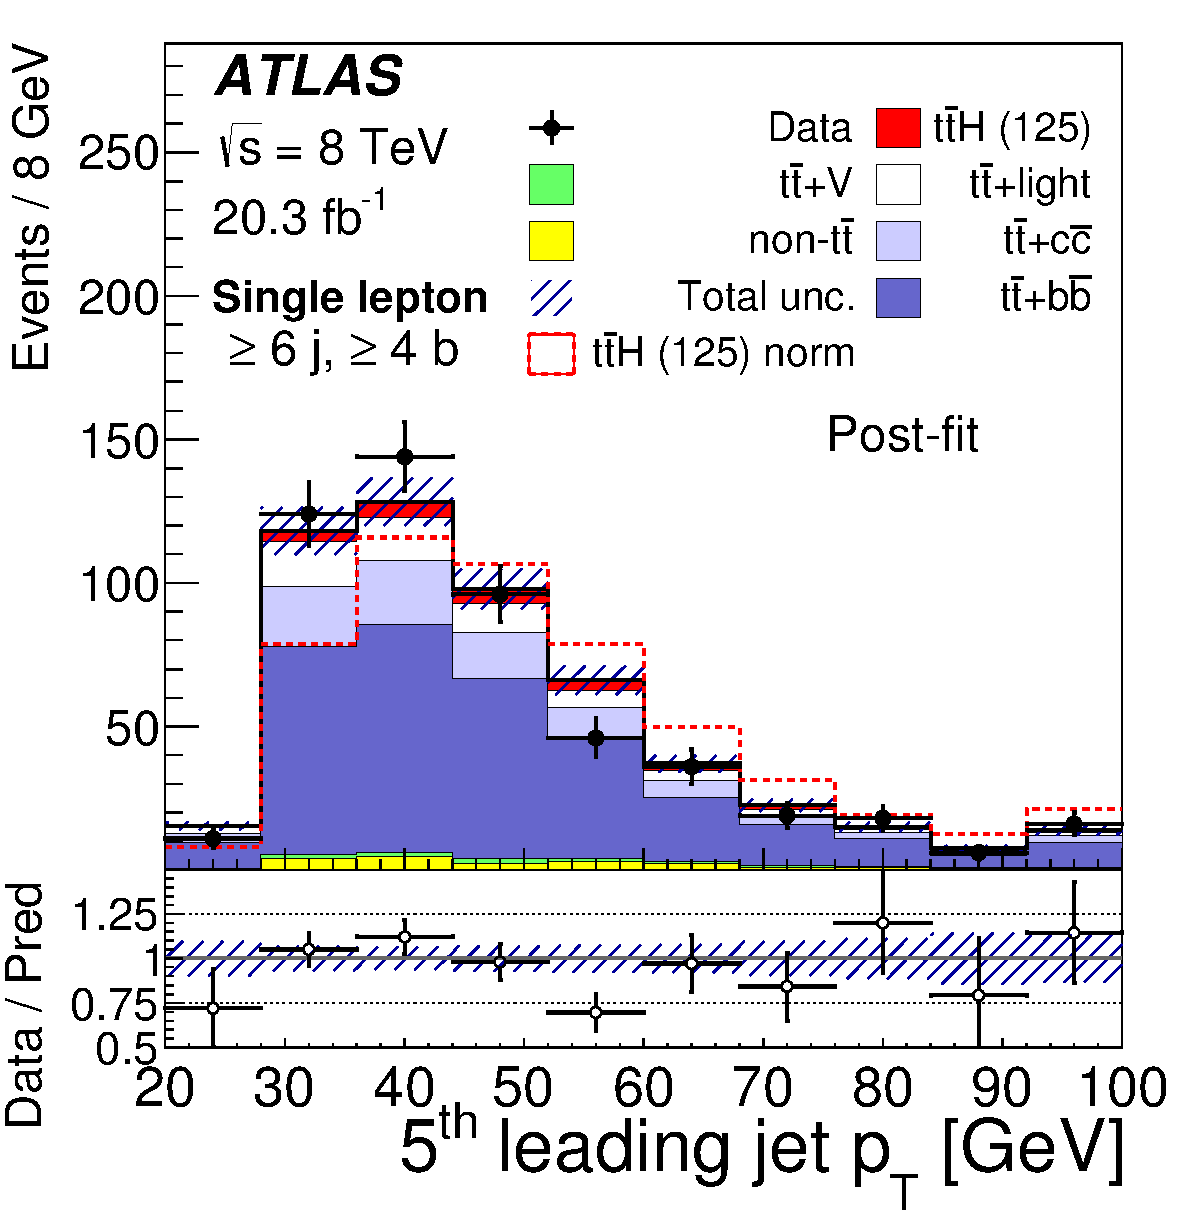
\includegraphics[width=0.49\textwidth]{Appendices/Figures_separation/jet5_pt_6jincl.pdf}
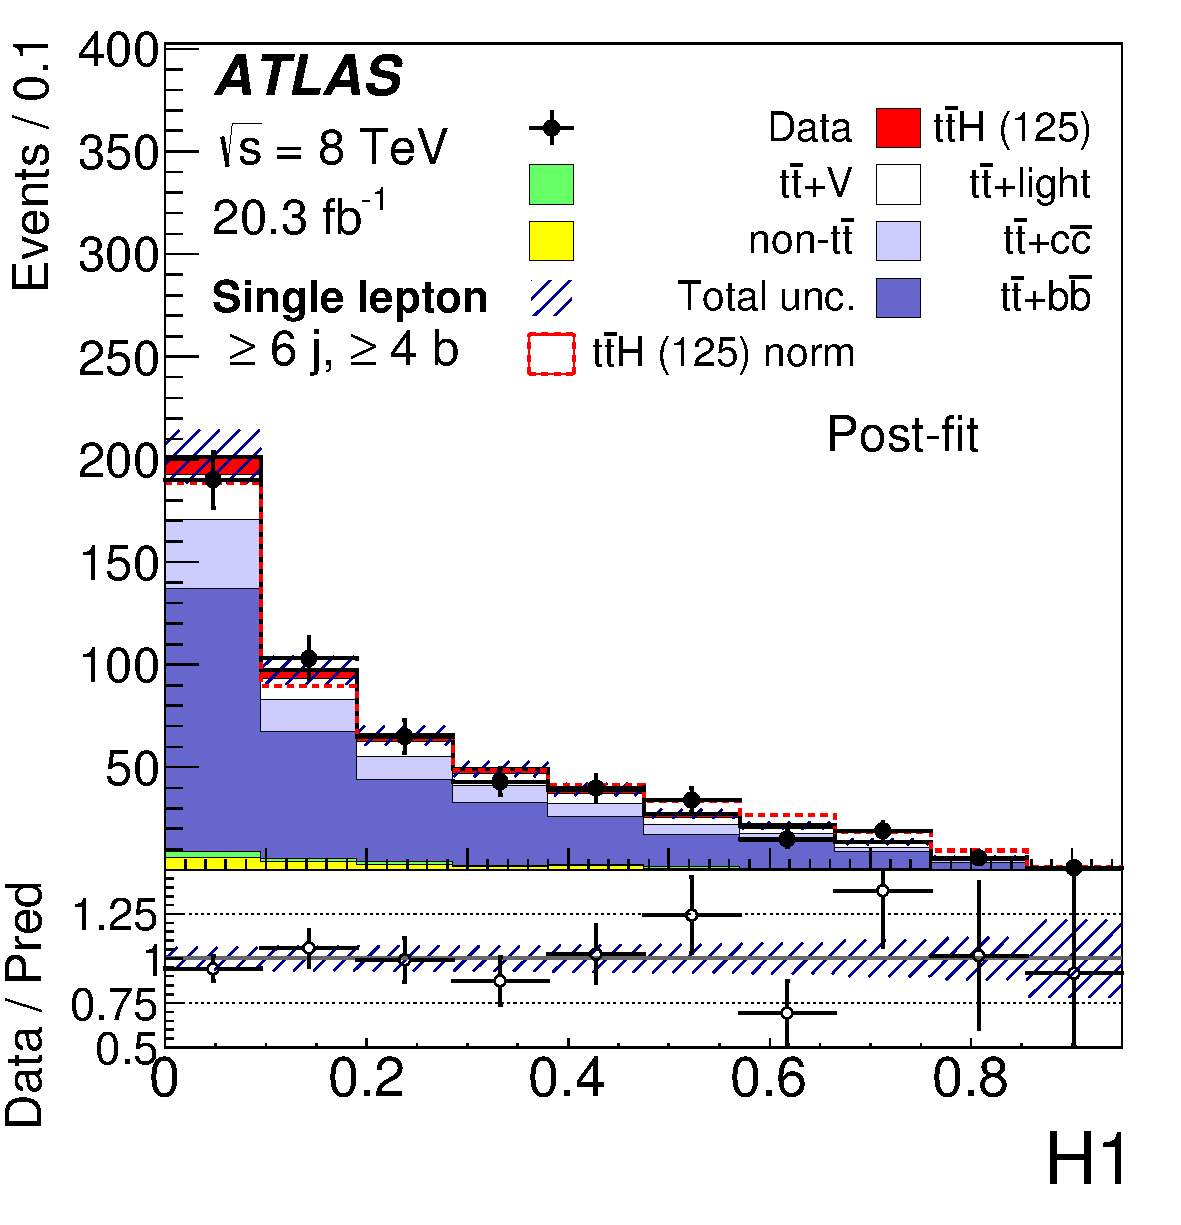
\includegraphics[width=0.49\textwidth]{Appendices/Figures_separation/H1_6jincl.pdf}
\caption{Post-fit comparison of data and prediction for the four top-ranked input variables in 
\sixfour\ region. The distributions shown are (a) $D1$, (b) \cent, (c) \ptjetfive, and (d) $H1$.
The first and last bins in all figures contain the underflow and
overflow, respectively. The bottom panel displays the ratio of 
data to the total prediction. The hashed area represents the uncertainty on the background.
The dashed line shows \tth\ signal
distribution normalized to background yield. The \tth\ signal yield (solid) 
is normalized to the fitted $\mu$.}
\label{fig:postinput_lj_3} 
\end{center}
\end{figure}
